%%% use twocolumn and 10pt options with the asme2e format
\documentclass[twocolumn,10pt]{asme2ej}
\newcommand{\gbf}[1] {\mbox{\boldmath${#1}$\unboldmath}}
\newcommand{\R}{\hbox{I \kern -.5em R}}
\usepackage{epsfig}
\usepackage{graphicx}
\usepackage{epstopdf}
\usepackage{color}
\usepackage{wrapfig}
\usepackage[hidelinks]{hyperref}
\usepackage{subfigure}
\usepackage{url}
\urlstyle{same}
\usepackage{caption}
\usepackage{algorithmicx}
%\usepackage{algorithm}
\usepackage{amsmath}
\usepackage[linesnumbered,ruled]{algorithm2e}


\hypersetup{
  colorlinks   = true, %Colours links instead of ugly boxes
  urlcolor     = blue, %Colour for external hyperlinks
  linkcolor    = blue, %Colour of internal links
  citecolor   = blue %Colour of citations
}

\newcommand{\nothing}{}
\newcommand{\req}[1]{(\ref{#1})}
\newcommand{\pos}[1]{\stackrel{+}{#1} \! }
\newcommand{\half}[1]{\frac{#1}{2}}
\newcommand{\nhalf}[1]{(\frac{#1}{2})}
\newcommand{\singleline}{\baselineskip 0pt}
\newcommand{\expo}[1]{exp$({\bf {#1}})$}

% Subfigure plot
\makeatletter
\newcommand{\putindeepbox}[2][0.7\baselineskip]{{%
    \setbox0=\hbox{#2}%
    \setbox0=\vbox{\noindent\hsize=\wd0\unhbox0}
    \@tempdima=\dp0
    \advance\@tempdima by \ht0
    \advance\@tempdima by -#1\relax
    \dp0=\@tempdima
    \ht0=#1\relax
    \box0
}}
\makeatother

% for displaying argmin command
\DeclareMathOperator*{\argminA}{arg\,min}

\def \Pluckerian{Pl\"uckerian }
\def \Plucker{Pl\"ucker }
\def \plucker{Pl\"ucker}
\def \Bezier{B\'{e}zier }
\def \BEZIER{B\'{E}ZIER }
\def \Shrocker{Schr\ddot{o}cker}

\title{A Machine Learning Approach to Kinematic Synthesis of Defect-Free Planar Four-Bar Linkages}
%%% first author
\author{Shrinath Deshpande,
    {\tensfb Anurag Purwar\thanks{Address all correspondence to this author at \href{anurag.purwar@stonybrook.edu}{anurag.purwar@stonybrook.edu}}}
    \affiliation{
    Computer-Aided Design and Innovation Lab\\
    Department of Mechanical Engineering\\
    Stony Brook University\\
    Stony Brook, New York, 11794-2300
    }
}

\begin{document}
\maketitle

%%%%%%%%%%%%%%%%%%%%%%%%%%%%%%%%%%%%%%%%%%%%%%%%%%%%%%%%%%%%%%%%%%%%%%
\begin{abstract}
Synthesizing  circuit-, branch-, or order- defects-free planar four-bar mechanism for the motion generation problem has proven to be a difficult problem. These defects render synthesized mechanisms useless to machine designers. Such defects arise from the artificial constraints of formulating the problem as a discrete precision position problem and limitations of the methods which ignore the continuity information in the input. In this paper, we bring together diverse fields of pattern recognition, machine learning, artificial neural network, and computational kinematics to present a novel approach that solves this problem both efficiently and effectively. At the heart of this approach lies an objective function which compares the motion as a whole thereby capturing designer's intent.
In contrast to widely used structural error or loop-closure equation based error functions which convolute the optimization by considering shape, size, position, and orientation of the given task simultaneously, this objective function computes motion difference in a form, which is invariant to similarity transformations. We employ auto-encoder neural networks to create a compact and clustered database of invariant motions of known defect-free linkages, which serve as a good initial choice for further optimization. In spite of highly nonlinear parameters space, our approach discovers a wide pool of defect-free solutions very quickly. We show that by employing proven machine learning techniques, this work could have far-reaching consequences to creating a multitude of useful and creative conceptual design solutions for mechanism synthesis problems, which go beyond planar four-bar linkages.


%The past forty years of research in mechanism synthesis has witnessed an unprecedented volume of work in formulating and solving planar four-bar linkage synthesis problems.
%However, finding practical and useful mechanisms for the motion synthesis problem has proven to be elusive, as a large majority of mechanisms turn out to be defective with respect to their assembly modes.
%Most methods formulate the problem as a discrete precision position problem, which inherently ignores the continuity information in the input, resulting in linkages with branch-, circuit- and order-defects.
%In this paper, we bring together diverse fields of pattern recognition, machine learning, artificial neural network, and computational kinematics to present a novel approach that solves this problem both efficiently and effectively.
%At the heart of this approach lies an objective function that compares the motion as a whole thereby capturing the designer's intent.
%In contrast to widely used structural error or loop-closure equation based error functions which convolute the optimization by considering shape, size, position, and orientation simultaneously, this objective function computes motion difference in a form, which is invariant to similarity transformations.
%We employ auto-encoder neural networks to create a compact and clustered database of invariant motions of known linkages.
%The query is raised in the database for nearest neighbors, which are either solutions or good initial conditions for fast local optimization techniques.
%In spite of highly nonlinear parameters space, our approach discovers a wide pool of defect-free solutions very quickly.
%We show that by employing proven machine learning techniques, this work could have far-reaching consequences to creating a multitude of useful and creative conceptual design solutions for mechanism synthesis problems, which go beyond planar four-bar linkages.

\textbf{keywords}: \emph{Machine Learning, Artificial Neural Network (ANN), Path Synthesis, Motion Synthesis, Planar Four-bar linkage, Circuit- Order-, and Branch-Defect}

\end{abstract}

\section{Introduction}
The mechanism synthesis problem deals with computing type and dimensions of a linkage system for performing specific tasks, which are often categorized as path, motion and function generation; see McCarthy and Soh \cite{sohmccarthy}, Sandor and Erdman~\cite{Sandor}, Hunt~\cite{Hunt78}, Hartenberg and Denavit \cite{Hartenberg},  Suh and Radcliffe \cite{Suh78}, and Lohse \cite{lohse2013}.
Path generation task aims to synthesize a mechanism which can guide a particular point of a rigid body (often, the coupler) along a prescribed path.
On the other hand, the objective of the motion generation task is to synthesize a mechanism which can guide a rigid body along a prescribed motion.
The prescribed path is given as a time sequence of positions, whereas the prescribed motion is given as a time sequence of positions and orientations. Various approaches have been proposed in the literature aiming to find acceptable solutions for path and motion generation problem. This paper is concerned with calculating the dimensional parameters of planar four-bar mechanisms while providing machine designers a robust set of defect-free solutions during the conceptual design phase, and thereby dramatically broadening the inventions design capabilities. 

A large majority of mechanism synthesis methods are based on the precision position approach.
This approach is a clever approximation trick to solve the above-mentioned problems, where the task is discretized into precision positions. These positions instead of the actual task, are required to be interpolated or approximated by the designed mechanism. However, this representation loses critical information about the actual continuous task and can lead to mechanisms with the order, circuit and branch defects; see Chase and Mirth\cite{chasemirth} for a thorough discussion on such defects. Unfortunately, these defects render mechanisms useless for their intended application.
\begin{figure}
\centering
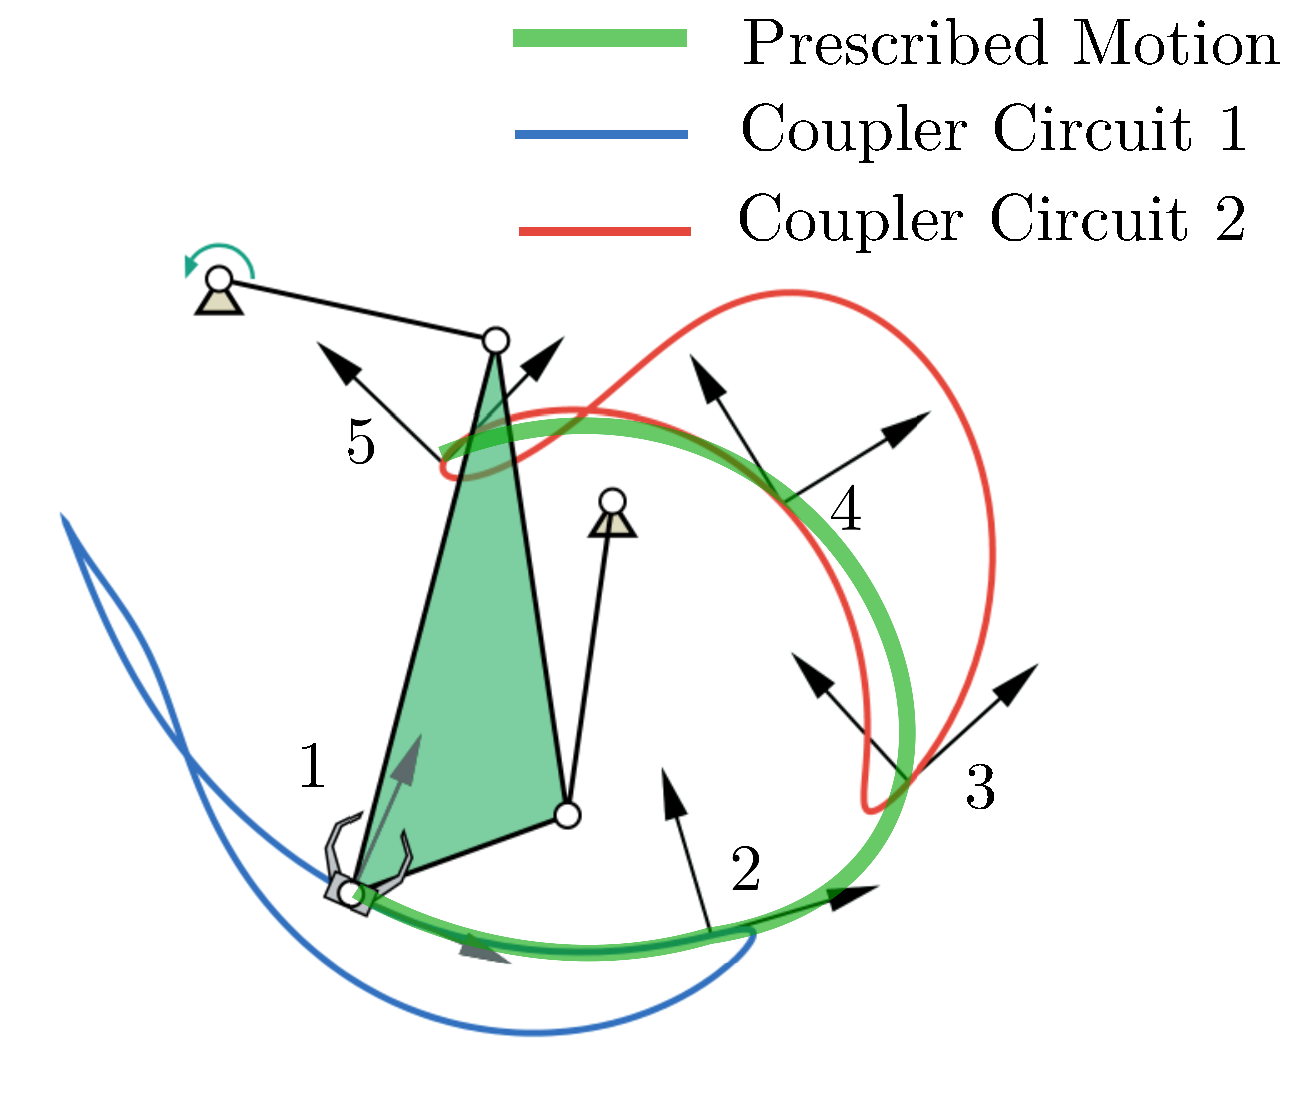
\includegraphics[width=200pt]{figure/fig_circuit_defect.eps}
  \caption{The four-bar mechanism obtained using the precision position approach suffers from circuit defect, as no coupler circuit passes through all precision positions.}
\label{circuit_defect}
\end{figure}
For an example, consider a motion generation problem shown in Fig.~\ref{circuit_defect}, where the objective is to synthesize a four-bar mechanism that can perform the prescribed motion going continuously from position 1 to 5. Instead of dealing with an infinite number of positions from initial to final one, currently this problem is simplified to design a four-bar that goes through all the five positions without any guarantee on the in-between motion. Burmester~\cite{Burmester86} showed that a four-bar can go through at most five precision positions and even in the best case scenario, there are a limited number of solutions. In this case, only one solution is obtained as shown in the Fig.~\ref{circuit_defect}. Although it can be seen that the coupler of the four-bar passes exactly through five precision positions, it can not do so without changing the circuit.
A circuit represents an assembly mode in which the mechanism is put together and to transition from one circuit to another, the mechanism has to be taken apart and reassembled. This phenomenon is called circuit defect in the linkage, which makes the linkage useless for the prescribed task.
To deal with it, an approach proposed in the literature is to tweak precision positions in a brute-force way within some tolerance until a solution is found.
Even if a circuit defect-free solution is found, the coupler motion in-between the precision points may go through undesired poses or in an incorrect order. This is an outcome of discarding the functional aspect of continuous motion and turning the problem into an interpolation problem bereft of important details. 

%As a guiding direction to advance state of the art, we propose the following criteria for an effective mechanism synthesis method,
%  \item \textbf{Data Driven}: The method should evolve by learning from its previous experiences, including providing quicker solutions for problems similar to previously solved problems.
%\end{enumerate}

% Global search methods
Instead of brute-force search within tolerance regions, some approaches apply separate constraints and form an optimization problem of non-differentiable objective function.
These methods employ metaheuristic algorithms like Differential-evolution (DE), Particle Swarm Optimization (PSO), Cuckoo Search (CS). Cabrera et al.\cite{Cabrera2002} used Genetic Algorithm for optimization in mechanism synthesis. Sardashti et al.\cite{sardashti2013} used PSO towards the defect-free synthesis of four-bar linkage with joint clearance for path generation problem. Ebrahimi and Payvandy\cite{Ebrahimi2015} presented an application of Imperialist Competitive Algorithm (ICA) for synthesizing path generating four-bars having desired workspace limits. Bulatovic\cite{Bulatovic2013} used Cuckoo Search for solving the problem of optimum synthesis of a six-bar double dwell linkage. 
%The above methods can produce many defect-free solutions and are scalable to any type of linkages. However, these methods tend to be slow and inefficient as they start from scratch for every instance with no guarantee of converging to an acceptable solution.

Path synthesis methods based on Fourier analysis do take the continuity information of coupler path into account.
However, most of them are defined only for closed loop curves.
Ullah and Kota\cite{ullah1997} have presented an invariant approach towards representation and synthesis of closed loop paths through shape optimization.
They use a combination of global and local search methods for optimizing Fourier Deviant function to compute the dimensions of planar four-bar linkages without an initial guess.
Wu et al.\cite{wu2011} presented a method based on finite Fourier series for open and closed path generation of four-bar mechanisms.
In the case of motion generation, Li et al.\cite{li2016} have developed a Fourier descriptor-based approach for approximate motion generation.
Bu$\acute{s}$kiewicz et al.\cite{Buskiewicz2009} used the curvature of the coupler curve for path synthesis using Genetic Algorithms.
Khan et al.\cite{khan2015} presented on approach where an artificial neural network is used for mapping between Fourier coefficients corresponding to a coupler path and corresponding linkage parameters.
% ---

% Atlas Based Methods ---
Instead of the global search, an alternative approach is to start from a good initial guess based on an atlas and use local search methods.
We adopt this approach and combine with our novel formulation to generate a diverse set of conceptual design solutions.
McGarva\cite{mcgarva1994} took the earliest approach towards creating a library for coupler trajectories based on the harmonic analysis.
Wandling\cite{wandling2000} has presented an atlas-based approach, where coupler paths and motions are stored in terms of Fourier Transforms.
Input motion is searched for neighbors based on Euclidean distances of Fourier Transforms.
Yue et al.\cite{yue-pathgen2011} presented a similar approach of path generation using P-Type Fourier Descriptor applicable for open curves.
In their approach, a task curve is transformed into normalized Fourier coefficients and queried for the nearest neighbor search.
The best match is returned as the solution to the input.
Chu et al.\cite{chu2010} presented an atlas-based method for synthesizing spatial four-bar linkages for function generation problems, where orientation data is stored in terms of Fourier descriptors.
\begin{figure*}
\centering
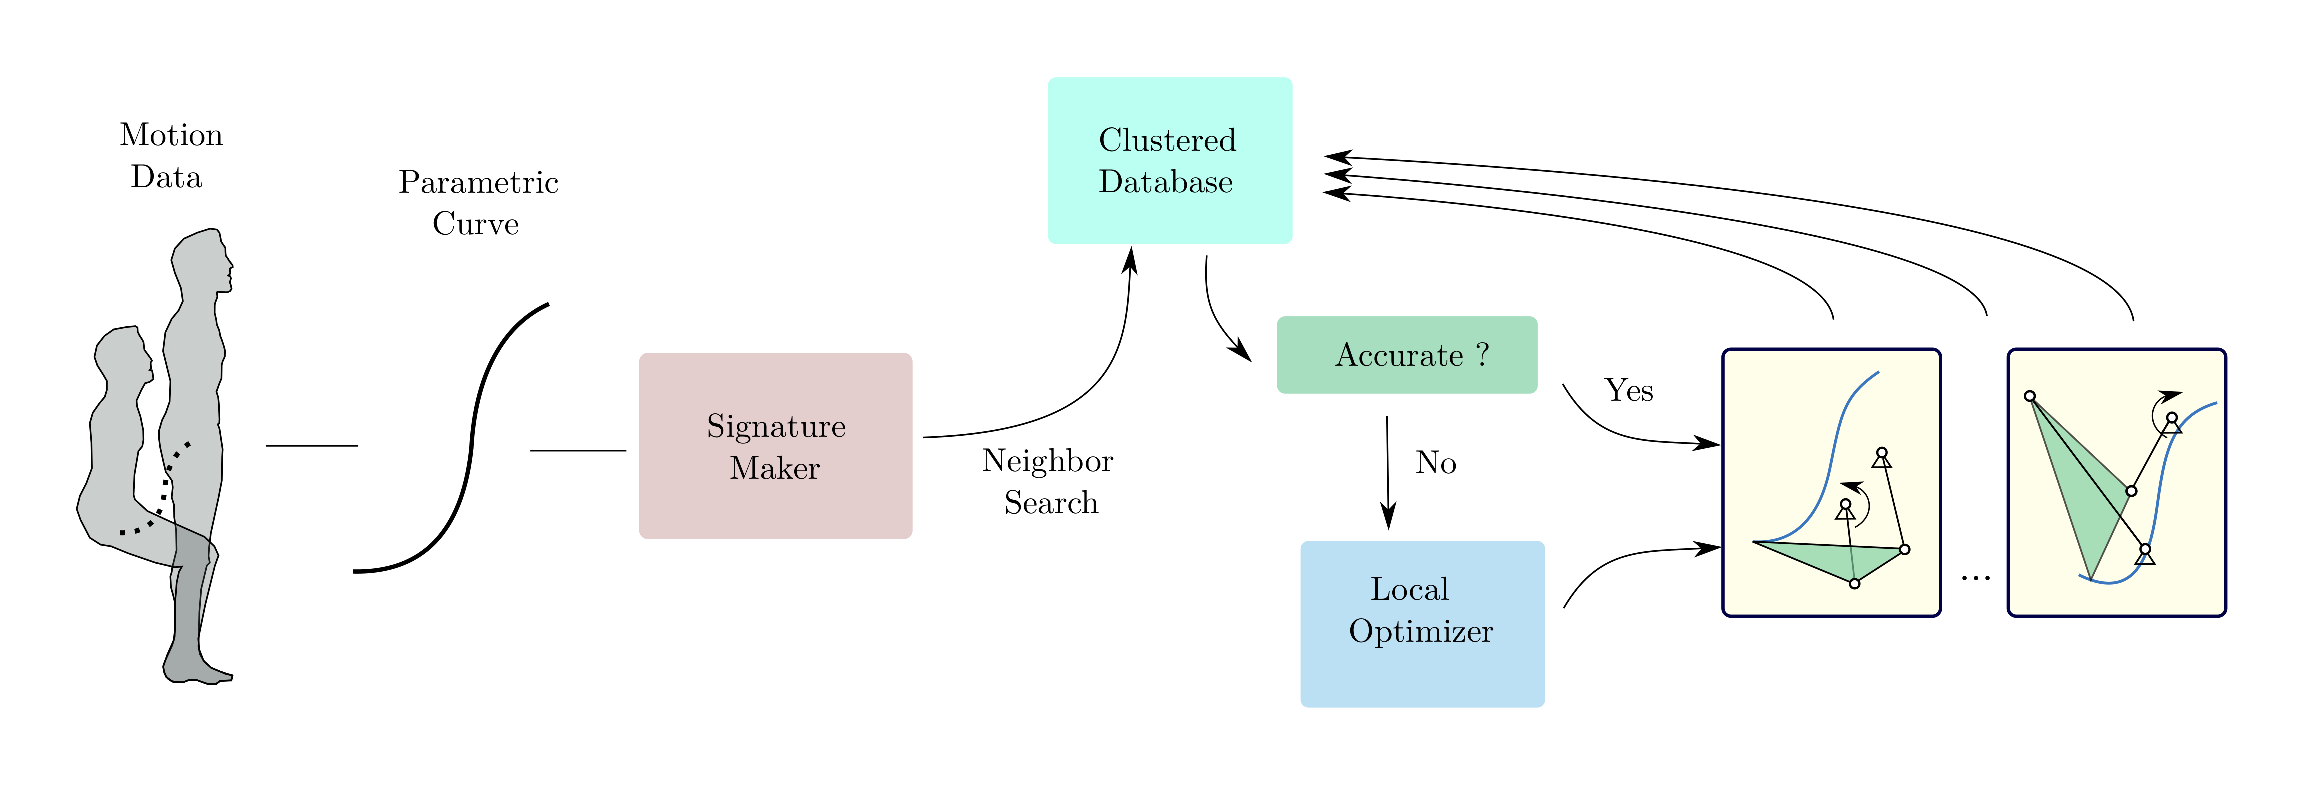
\includegraphics[width=\textwidth]{figure/overall_approach.eps}
  \caption{The Machine Learning approach begins by creating an invariant signature for the path and the motion data, which facilitates a compact and hierarchical clustered database and an auto-encoder Neural Network trained to elicit good, defect-free solutions or subjected to local, fast optimization. The results are defect-free conceptual design solutions for input problems.}
\label{overallMethod}
\end{figure*}
The above methods generate data based on uniform sampling in the linkage parameter space.
Given the highly nonlinear mapping between linkage parameters and coupler trajectory, this way of sampling leads to a nonuniform sampling of trajectory space, which causes under-representation of possible motions.
We address this issue by employing log-normal distribution in the linkage parameter space to generate the data samples.
Then, we perform a compact clustering of the data using machine learning techniques.
A hierarchy is created in the database by means of clustering, where the top level comprises of data points called cluster centers, which are representative of the cluster points in lower levels.
Wandling~\cite{wandling2000} and Yu et al.~\cite{yue-pathgen2011} have built libraries with all possible coupler curves, where one curve is broken down into many segments for creating data for partial curves.
In contrast to this, we need to store only one curve that represents all the segments in it.
This is because our representation facilitates part-to-whole matching.
None of the other previous methods facilitate this partial matching of open motion curve into another open or closed curve, which significantly contributes to providing a large number of solutions, and reduces the data requirement even further.
%  ---

In this paper, we represent the given task as a parametric continuous function of poses or path-points. The objective is to find a linkage which has a coupler motion or path compatible with the given task. We develop a compatibility measure invariant to similarity transformations so that position, scaling, and orientation of the given path or motion do not convolute the optimization.
Next step is to conduct a search in the space of linkage parameters to find linkages with coupler motions compatible with the prescribed task.
Although global search methods can be applied for finding solutions, we employ an efficiently clustered database and Powell's local search method to come up with a variety of different solutions.
The motivation behind using a clustered database is rooted in the broader objectives of machine design. Mechanism synthesis is a critical part of the conceptual design phase, which requires synthesis method to be prolific in terms of concept generation to 1) realize the potential of attainable design possibilities, and 2) have the agility to adapt a design to evolving requirements.
Our method only deals with the coupler curves and is not dependent on the linkage type.
Thus, it is readily scalable to any type of planar linkage.

The synthesis routine starts by creating a continuous parametric representation of a prescribed path or motion. We employ pattern recognition and computational shape analysis to create an invariant signature for the prescribed path and motion.
A query representing an invariant signature of the prescribed path or motion is raised for $k$ nearest neighbors among cluster centers in the database.
These $k$ neighbors, if needed, are subjected to fine-tuning by local optimization to obtain a set of defect-free solutions.
The objective function that drives the synthesis process computes a distance measure of dissimilarity between the task and the coupler motion or path generated by current linkage parameters.
This distance measure of dissimilarity inherently requires continuity of motion, thus ensuring that the output mechanism is defect-free throughout the task.
Figure~\ref{overallMethod} illustrates an overview of our method, which is codified in Algorithm~\ref{alg_overall}.

The original contributions of the paper are in 1) creating a perceptive problem formulation for path and motion generation, which solves the issues associated with the precision position approach,
%The formulation is based on a measure of dissimilarity between two planar motions or paths, which is invariant to similarity transforms.
2) exploiting the nonlinear nature of the relationship between the linkage parameters and coupler motions to create a sensitive, wide-ranging, compact, and efficient database with hierarchical clustering, and 3) developing a novel algorithm for partial matching of motions and paths which significantly improves the synthesis. 

%In this paper, we 1) employ pattern recognition and computational shape analysis to create a similarity Transform-independent signature for coupler path and motion, 2) exploit the nonlinear nature of relationship between the linkage parameters and coupler motions to create a sensitive, wide-ranging, compact, and efficient database with hierarchical clustering, and 3) enable dimensionality reduction using Auto-encoder Neural Networks.

Rest of this paper is organized as follows. Section~\ref{sec_sign} presents the computation of motion and path signatures.
Section~\ref{sec_distanceMetric} is comprised of evaluation criterion for signatures based on the shape similarity, which leads to the formulation of error function for optimization.
Section~\ref{sec_SA} discusses the nature of objective function via sensitivity analysis at a singularity.
Section~\ref{sec_db_ae} presents the database generation and clustering using auto-encoders for efficient sampling and query operations.
Finally, two case studies are presented in section~\ref{sec_example} to illustrate the efficiency and efficacy of the method.
%%%%%%%%%%%%%%%%%%%%%%%%%%%%%%%%%%%%%%%%%%%%%%%%%%%%%%%%%%%%%%%%%%%%%%

\begin{algorithm}
    \SetKwInOut{Input}{Input}
    \SetKwInOut{Output}{Output}
    \Input{Task Motion $\{x_i,y_i,\theta_i\}_{i=1}^{N}$ or Path$\{x_i,y_i\}_{i=1}^{N}$ }
    \Output{Linkage Parameters \emph{\textbf{l}: $l_1$, $l_2$, ...}}
    signature = calculateSignature(Input); \\
    distances = [];\\
    \For{centerPoint \textbf{in} clusterCenters}
    {
      distances.push(getDistance(signature, centerPoint))
    }
    $k$Neighbors = getNeighbors(distances, $k$)
    \For{neighbor \textbf{in} kNeighbors}
    {
      \eIf{threshold $<$ neighbor.distance}
      {
        \textbf{return} $neighbor.LinkParameters$
      }
      {
        \textbf{return} Optimize$(neighbor.LinkParameters)$
      }
    }
    \caption{Planar Linkage Synthesis}
    \label{alg_overall}
\end{algorithm}

%%%%%%%%%%%%%%%%%%%%%%%%%%%%%%%%%%%%%%%%%%%%%%%%%%%%%%%%%%%%%%%%%%%%%%
\section{Signatures of Coupler Path and Motion}\label{sec_sign}
Focus of the paper is on a novel method for mechanism synthesis that takes a parametric motion $(x:x(t), y:y(t), \theta:\theta(t))$ or path $(x:x(t), y:y(t))$ as the input, and returns defect-free linkages that produce similar motion or path.
The input is transformed into a representation, termed as a signature, which is invariant to similarity operations, viz. reflection, rotation, translation, and scaling.
Signatures for path and motion are termed as path signature and motion signature, respectively.
For calculating the path signature, we use the formulation developed by Cui et.al\cite{cui2009}.

Consider a motion given in parametric form as, $x:x(t), y:y(t), \theta:\theta(t)$, where $\theta(t)$ is the change in orientation along the path with respect to initial orientation.
It should be noted that $\theta(t)$ is a continuous curve with domain ($-\infty$, $\infty$) in contrast to conventional domain i.e. [$-\pi$, $\pi$].

Curvature $\kappa(t)$ of the path $(x:x(t), y:y(t))$ and its integral $K(t)$ is given by,
\begin{eqnarray}
  \kappa(t) = \frac{\ddot{y}(t)\dot{x}(t) - \ddot{x}(t)\dot{y}(t)}{{(\dot{x}^2(t) + \dot{y}^2(t))}^{(\frac 32)}}, \label{curvatureEq}\\
  K(t) = \int^{t}_0 |\kappa(t)|dt \label{kInt},
\end{eqnarray}
where $\dot{x}(t)$, $\ddot{x}(t)$ are first and second order derivative with respect to parameter $t$.
As an example, the parametric motion could be a B-spline motion as shown in Fig~\ref{bsplineFitting}.
We compute $\kappa(t)$ and $K(t)$ along the direction of $t$ using Eq.~\req{curvatureEq} and Eq.~\req{kInt}, respectively.
Figure~\ref{curvatureK} shows computed curvature and its unsigned integral for the coupler path shown in the Fig.~\ref{bsplineFitting}.
It can be seen that the curvature is small at the start, increases as the curve bends along the path and drops once again as the path straightens out. It is obvious that the curvature plot will reverse if the direction of parameterizations reverses, while the integral is a monotonically increasing function.

\begin{figure}
\centering
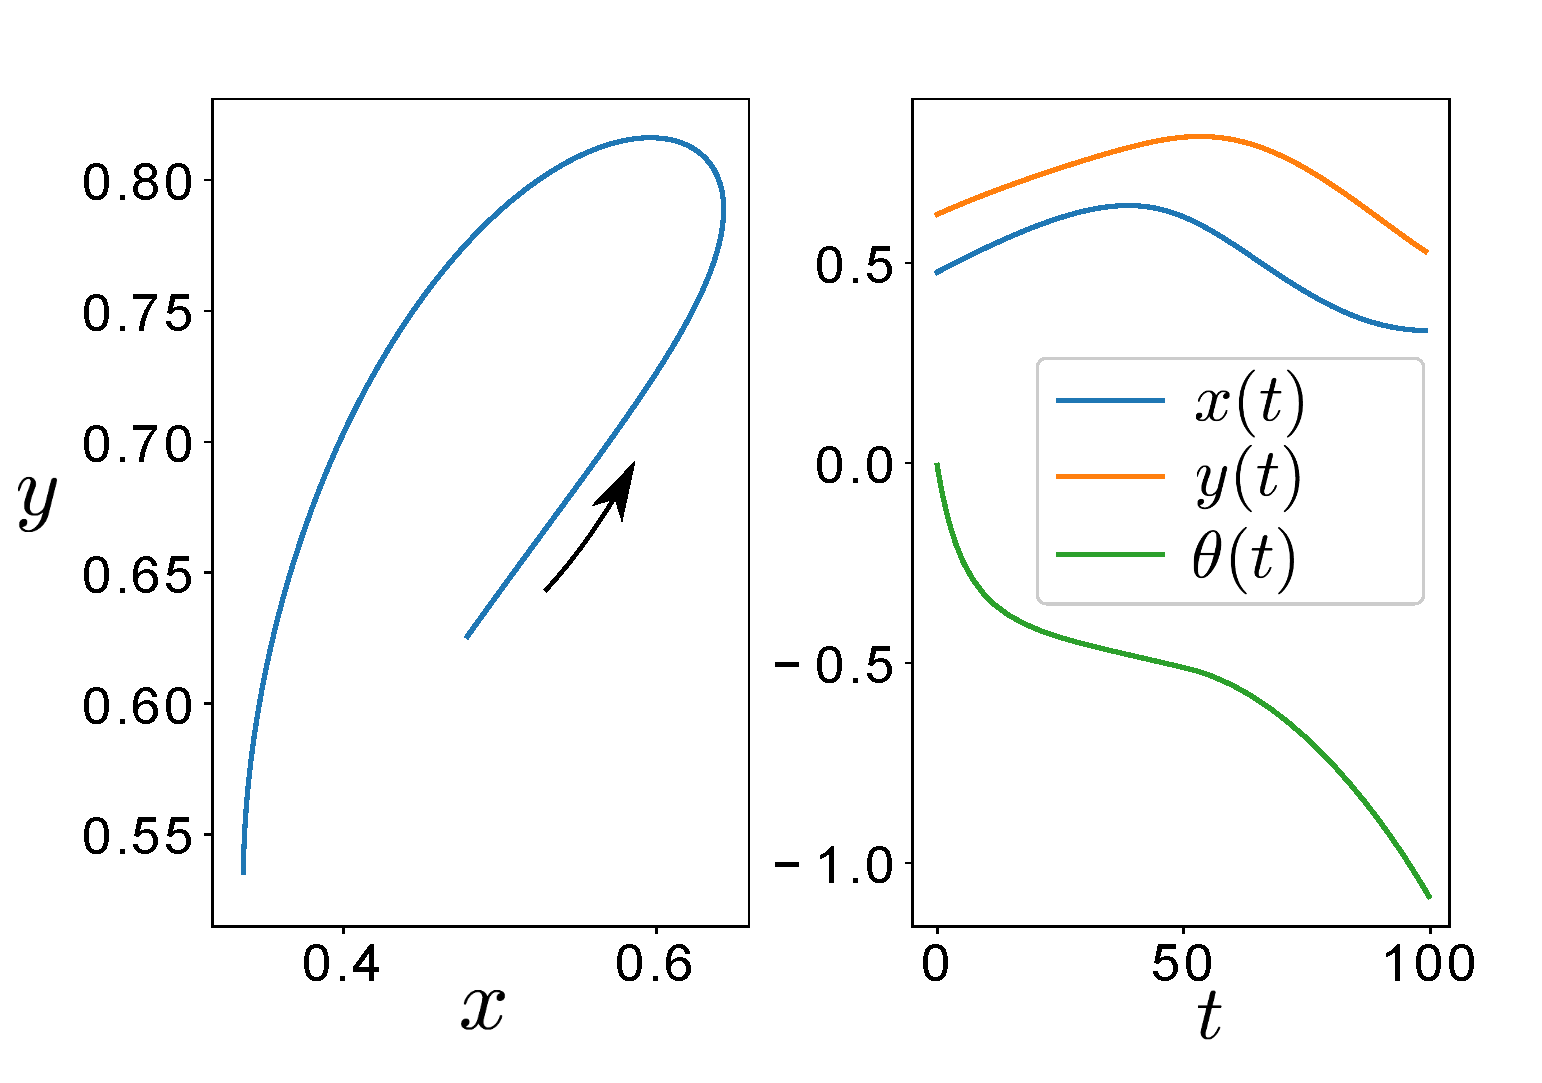
\includegraphics[width=240pt]{figure/fig_bspline.eps}
  \caption{a) The path of the input motion along with direction of parametrization, b) motion components $x(t), y(t), \theta(t)$ are plotted against parameter t.}
\label{bsplineFitting}
\end{figure}

\begin{figure}
\centering
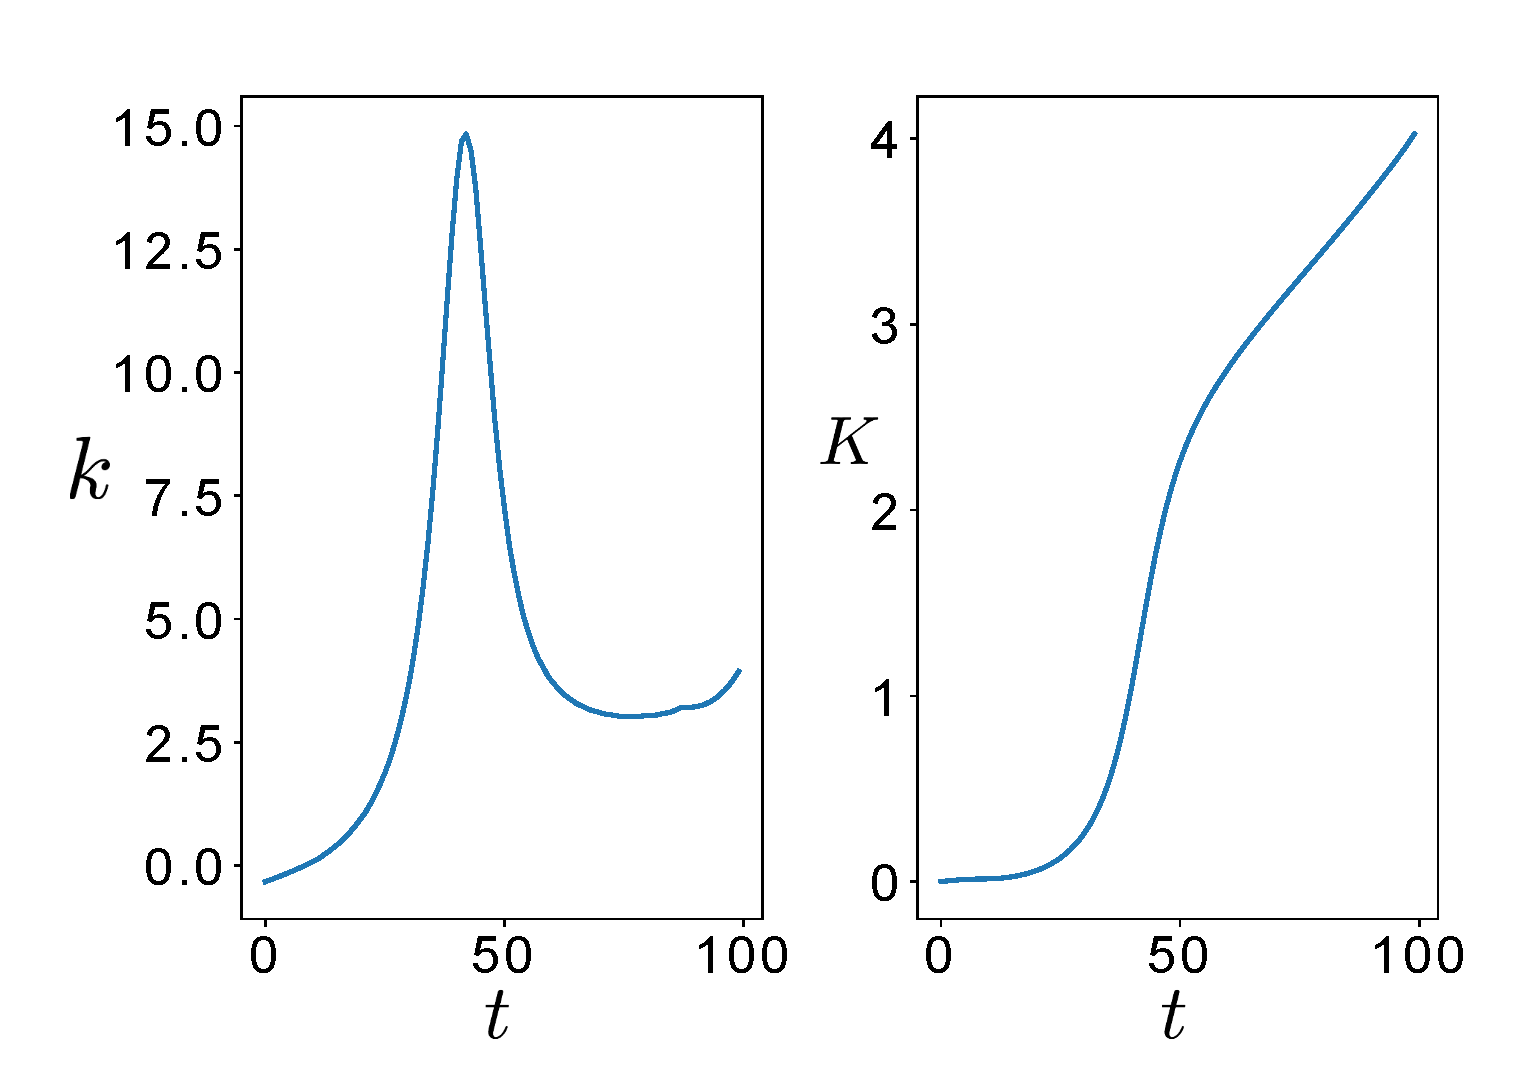
\includegraphics[width=240pt]{figure/fig_curvatureK.eps}
  \caption{Curvature and its unsigned integral for the path shown in Fig.~\ref{bsplineFitting}}
\label{curvatureK}
\end{figure}

Now, we re-sample the curvature at equal intervals of $K(t)$, which is equivalent to plotting $\kappa$ vs $K$ in Fig~\ref{signature}(a).
This is done by finding the parameter values of $t$ where $K$ changes uniformly.
For practical purposes, we find an array of the parameter $t$ such that $K$ increments by 0.1.
For each value of $t$ in that array, we compute $\kappa(K)$ and $\theta(K)$ and store it as the path and motion signatures respectively.
We note that there is a one-to-one mapping between $t$ and $K$.
Although it may seem natural to use planar quaternions~\cite{McCarthy90, Bottema} for representing motion and finding its signature, it couples orientation with the path in such a way that the signatures formed no longer remain invariant to similarity transformation.

These signatures are invariant under similarity transformations; for proof see\cite{cui2009}.
We know that curvature changes inversely to the scale of the curve, so when it is integrated along the scaled curve, the scale factor cancels itself out. Reflection operation produces flipped path signature, but motion signature remains invariant.
Figure~\ref{signature} shows the path and motion signature obtained for the motion depicted in Fig.~\ref{bsplineFitting}. It is important to note that the signature depends on the direction of parameter $t$.
The procedure of signature calculation presented in this section is given in the Algorithm ~\ref{alg_signature}.

\begin{figure}
\centering
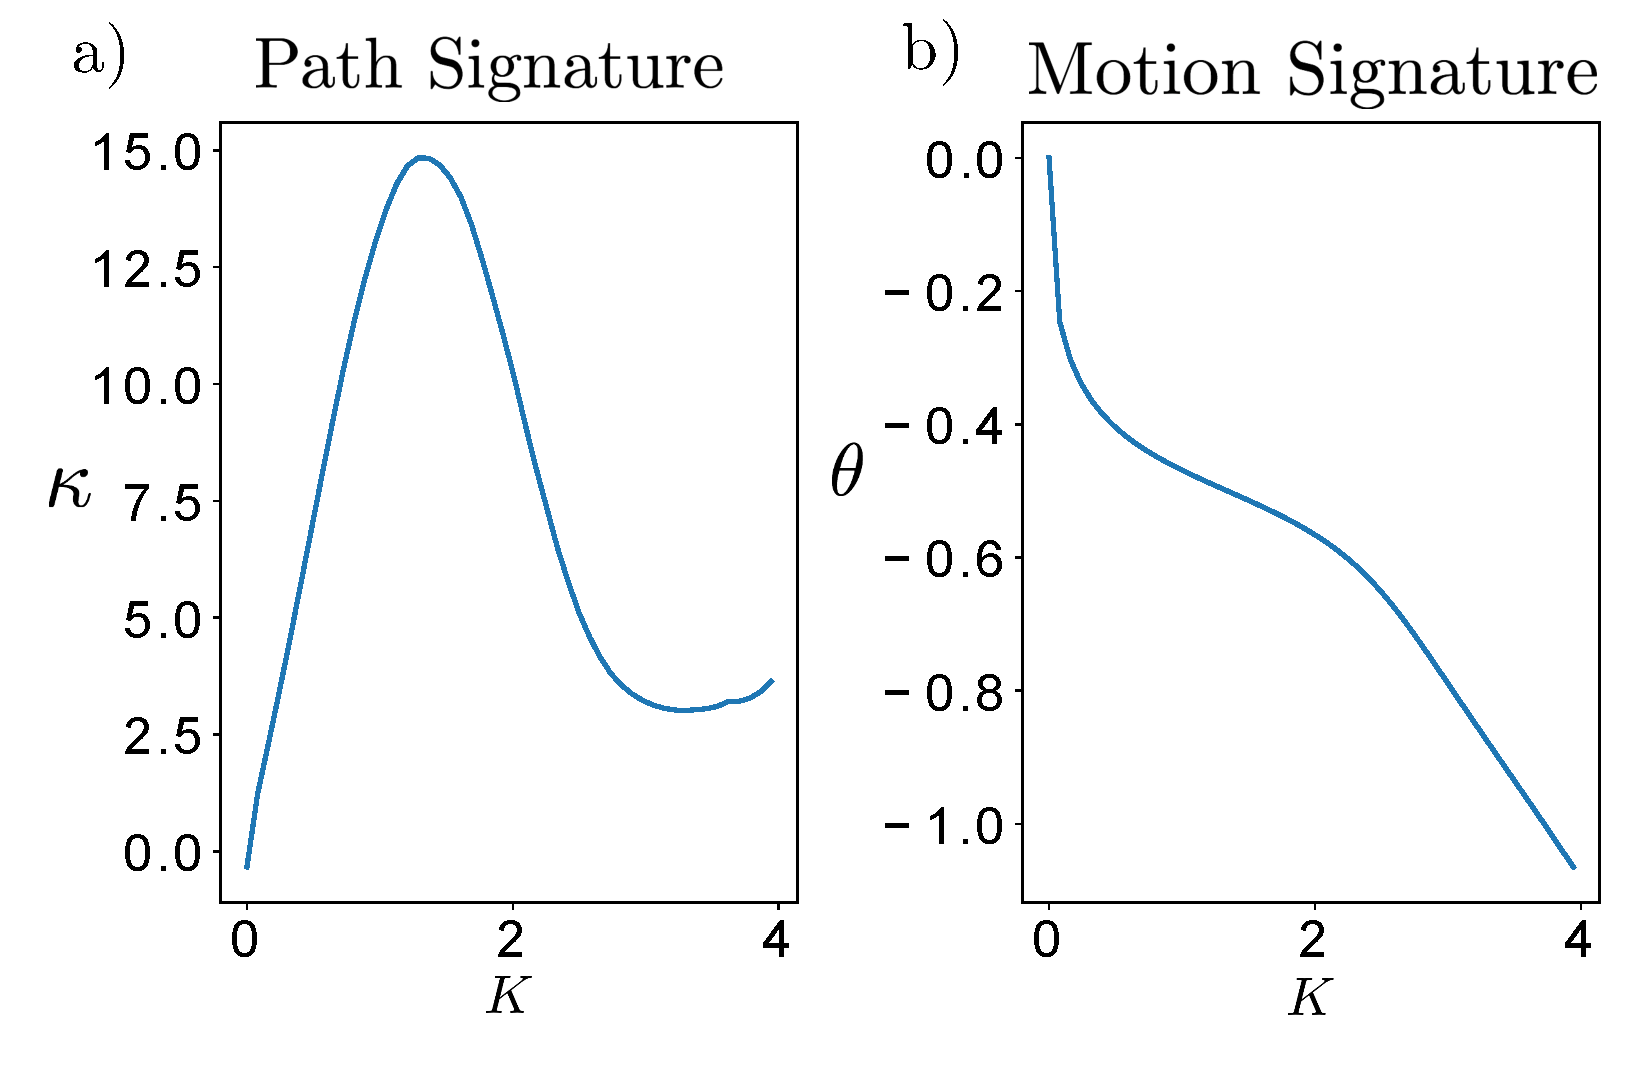
\includegraphics[width=240pt]{figure/fig_signatures.eps}
  \caption{Path and motion signatures of the motion shown in Fig.~\ref{bsplineFitting}}
\label{signature}
\end{figure}


\begin{algorithm}
    \SetKwInOut{Input}{Input}
    \SetKwInOut{Output}{Output}
    \Input{Twice Differentiable Parametric Representation of Motion $(x:x(t), y:y(t), \theta:\theta(t))$}
    \Output{signature //discretized signal in form of an array}
    $\kappa(t)$ = ComputeCurvature$(x, y)$ using Eq.~\ref{curvatureEq} \\
    $K(t)$ = IntergrateCumulatively($\kappa(t)$) using Eq.~\ref{kInt} \\
    motionSignature = [] \\
    pathSignature = [] \\
    \For{$i = 0 \to max(K)$}
    {
      $tmp$ = (value of $t$ corresponding to which $K$ has value $i$) \\
      $i = i + 0.1$ \\
      motionSignature.push($\theta$($tmp$)) \\
      pathSignature.push($\kappa$($tmp$))
    }
    \Return{PathSignature, MotionSignature}
    \caption{Calculate Invariant Signatures}
    \label{alg_signature}
\end{algorithm}

\section{Signature Matching and Error Function}\label{sec_distanceMetric}
The signatures obtained in previous steps contain important information about the shape of the trajectory.
In this section, we formulate functions that evaluate the similarity between two trajectories based on their signatures.
These distance functions can be used as an error metric, which can be minimized using optimization methods.

\subsection{Partial Matching of Path Signatures}\label{sec_ncc}
When a path query is raised, it can be very useful to know whether this path matches with a part of a path from the database.
This subsection presents a method for determining this partial similarity.

Let us consider two coupler paths; namely \emph{Part} and \emph{Whole} as shown in Fig.~\ref{wholePart}.
Let $p$ and $W$ be their signatures respectively, where $W$ completely contains $p$ as shown in Fig.~\ref{pathSignature}.
The orientation information shown in Fig.~\ref{wholePart} is ignored for path matching. It will be used later for matching of motion signatures.
The partial matching works as follows:

\begin{enumerate}
  \item $p$ and $W$ are expressed in terms of arrays and $W$ must contain more points than $p$.
  \item $p$ is slided with offset index $j$ along $W$.
  \item For each offset $j$, we compute normalized cross-correlation function~\cite{lewis1995fast}  given by,
\end{enumerate}
\vspace{-0.6cm}
\begin{equation}\label{nccEq}
  Cn(j, p, W) = |\sum_{i}^{p_{sp}} \frac{(W(i+j) - \bar{W}(j : j + p_{sp}))(p(i) - \bar{p})}{\sqrt{\sum_{i}^{p_{sp}}{(W(i+j) - \bar{W}_{p_{sp}})}^2\sum_{i}^{p_{sp}}{(p(i) - \bar{p})}^2}} |,
\end{equation}
where $Cn(j, p, W)$ is the normalized cross-correlation value when $p$ is matched against $W$ at $j^{th}$ index; $p_{sp}$ is length of the array $p$ and $\bar{W}(j:j + p_{sp})$ is mean of the values of array $W$ between index range of ($j, j+p_{sp}$).

Here, $p$ acts as a template that tries to find the best match against $W$ while sliding over it along $j$.
Domain of $Cn(j, p, W)$ is [0, 1], where 1 represents the complete embedment of $p$ inside $W$, i.e., \emph{Part} is identical to a portion of \emph{Whole}.

The maximum score of the matching $Cn_{max}(p, W)$ represents similarity of the template in $W$, and offset index $j$ at which maximum occurs is the starting point for matching.
As we know that the signature reverses with reversal of the direction of $t$, we compute the correlation along both directions and select the best matching score, offset index and the matching direction of sampling.
Figure~\ref{ncc} depicts normalized cross correlation function over the sliding domain $j$ for \emph{Part} and \emph{Whole} curves.

\begin{figure}
\centering
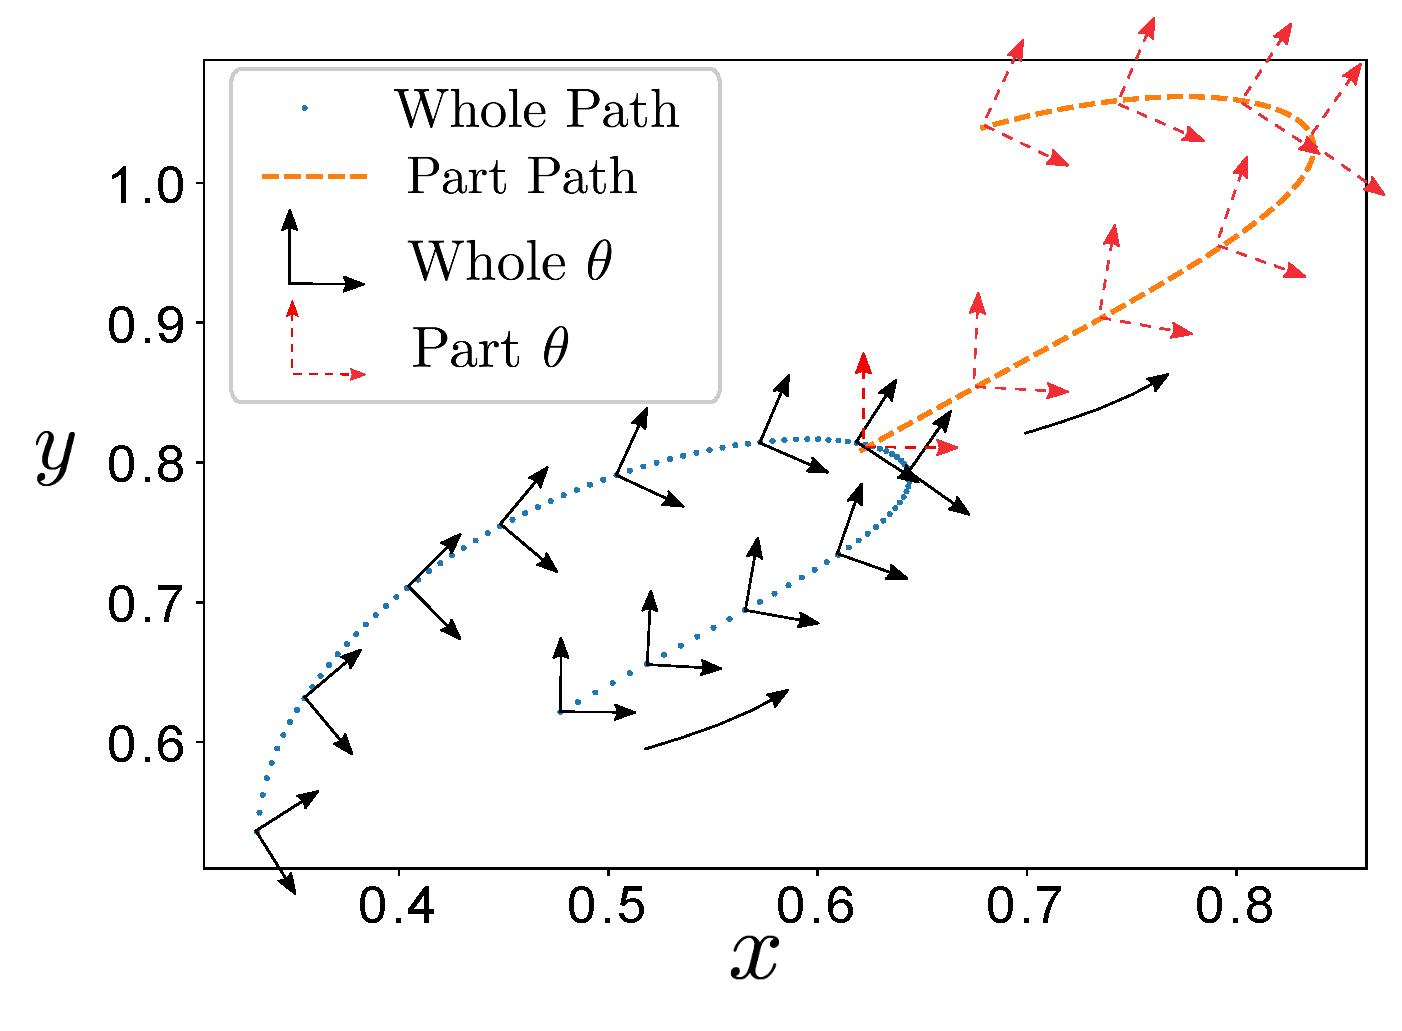
\includegraphics[width=240pt]{figure/fig_whole_part.eps}
  \caption{\emph{Part} path is formed by trimming whole path followed by translation and scaling. Arrows indicate the increasing direction of parameter $t$.}
\label{wholePart}
\end{figure}

\begin{figure}
\centering
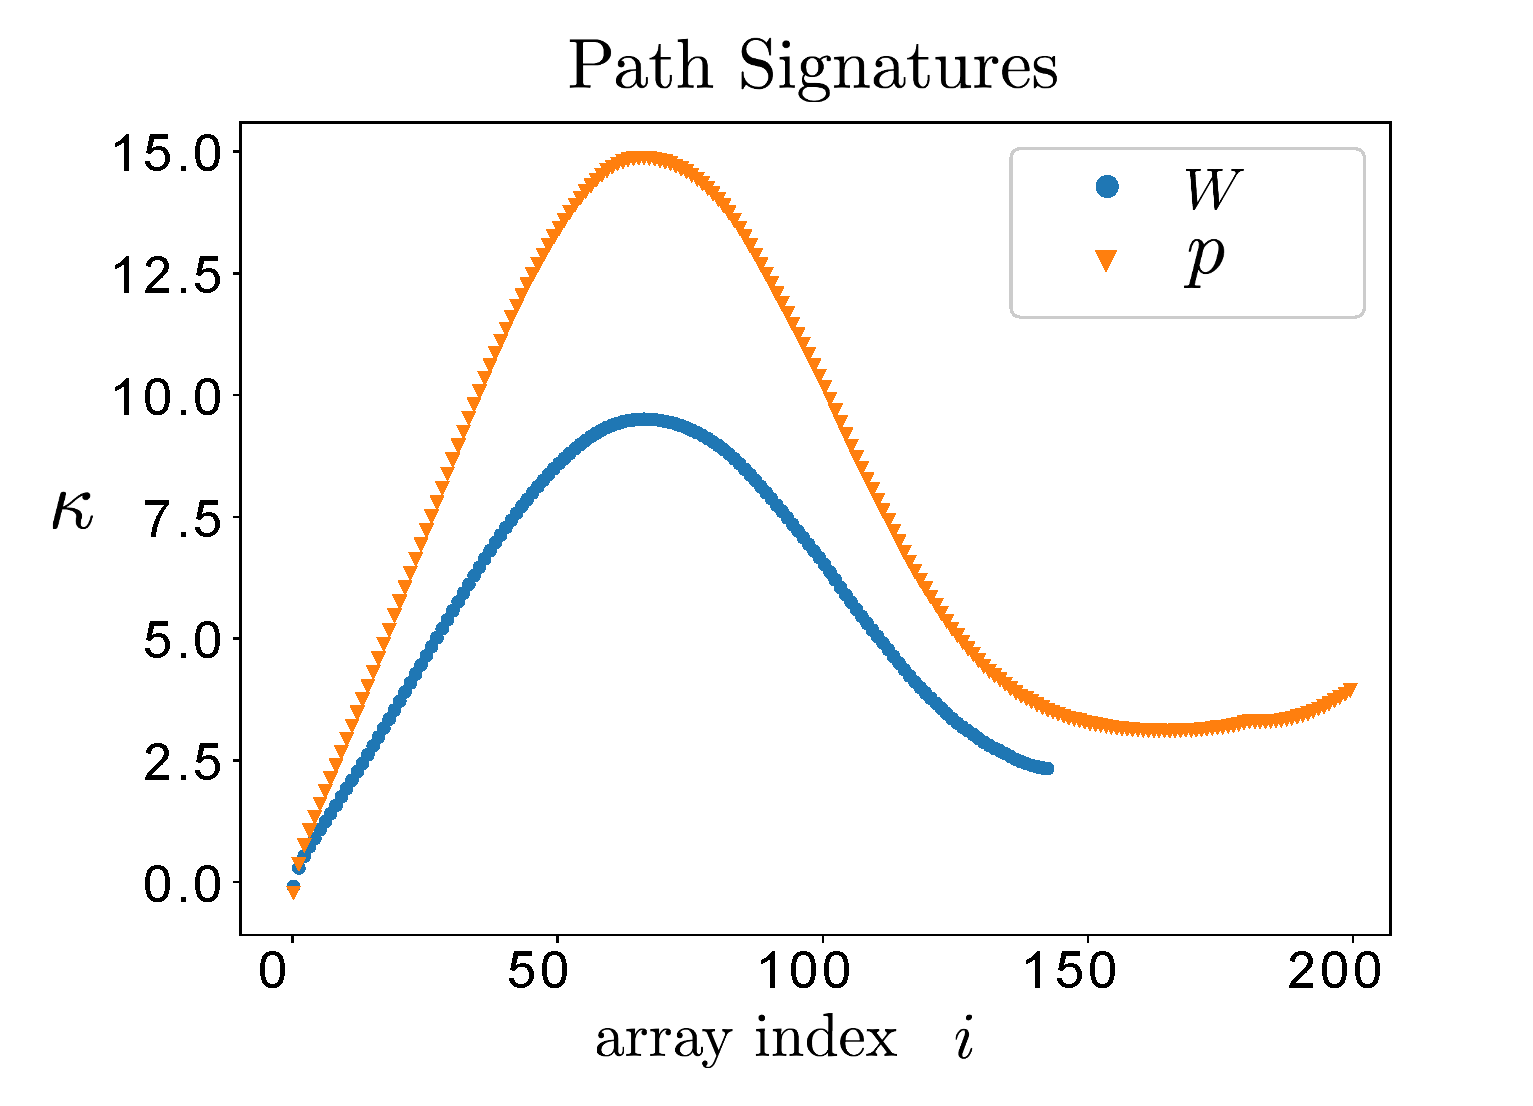
\includegraphics[width=240pt]{figure/fig_path_signatures.eps}
  \caption{Path Signatures of part $p$ and whole $W$ from the Fig.~\ref{wholePart}. The array index $i$ corresponds to the index location for the array of the $K$. The domain of path signature is scale-invariant but the range still has a scaling factor, which is taken care of by normalized cross-correlation.}
\label{pathSignature}
\end{figure}

\begin{figure}
\centering
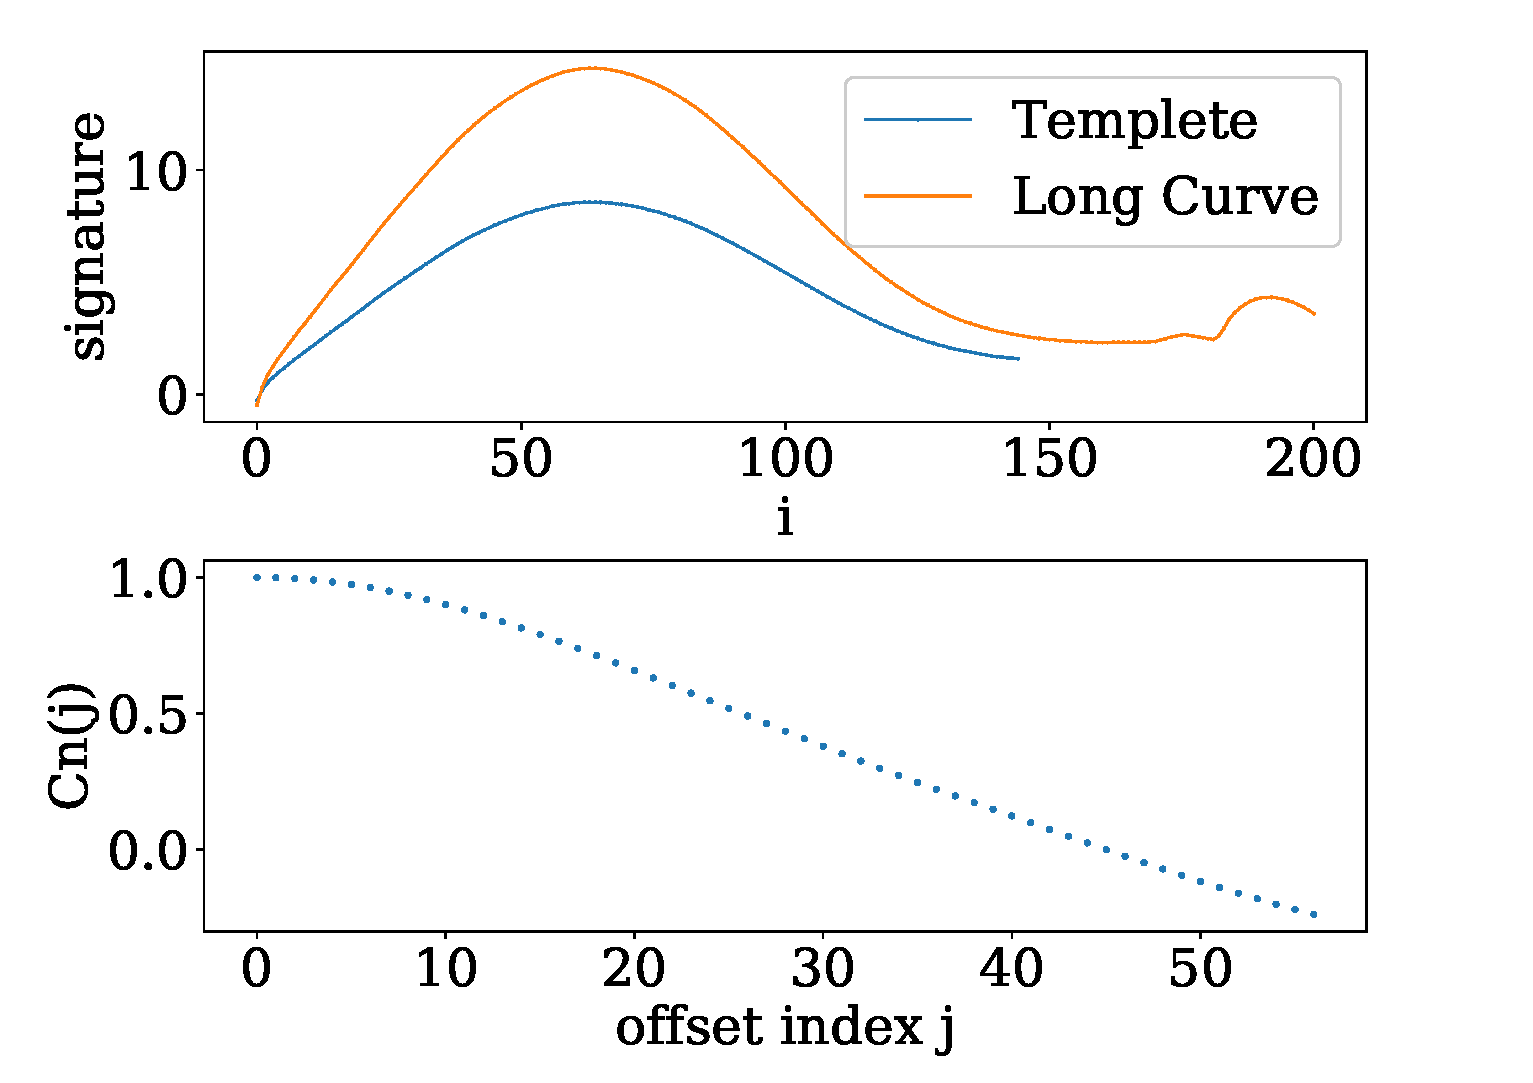
\includegraphics[width=240pt]{figure/fig_ncc.eps}
  \caption{Normalized cross correlation of the signatures computed along each direction is shown. It can be seen that exact match is found at $j=0$.}
\label{ncc}
\end{figure}

\subsection{Partial Matching of Motion Signatures}\label{sec_mcc}
This section presents how a template motion can be checked against other motion for potential matching.
Consider \emph{Part} and \emph{Whole} motions shown in Fig.~\ref{wholePart}.
Let $p$ and $W$ be the motion signatures of the \emph{Part} and \emph{Whole} motions, respectively as shown in Fig.~\ref{motionSignature}.
Similar to partial matching of path signatures, the cross-correlation function is given by,

\begin{equation}\label{mccEq}
  E(j, p, W) = \sum_{i}^{p_{sp}} {((W(i+j) - \bar{W}(j: j + p_{sp})) - (p(i) - \bar{p}))}^2,
\end{equation}
where $E(j, p, W)$ is the dissimilarity value when template $p$ is matched to $W$ at $j^{th}$ index. Here $p$ tries to find the best match against $W$ while sliding over it.
Similar to path signature, motion signature is dependent on the direction of $t$. Thus, we compute the dissimilarity for both directions and choose whichever is the least, i.e., $E_{min}(p, W)$.
Figure~\ref{mcc} depicts dissimilarity function over the sliding domain $j$.
In this case, as shown in Fig.~\ref{mcc}, we find that the first point is the matching point, which is consistent with the fact that we have essentially sliced the whole motion to obtain the part motion.

\begin{figure}
\centering
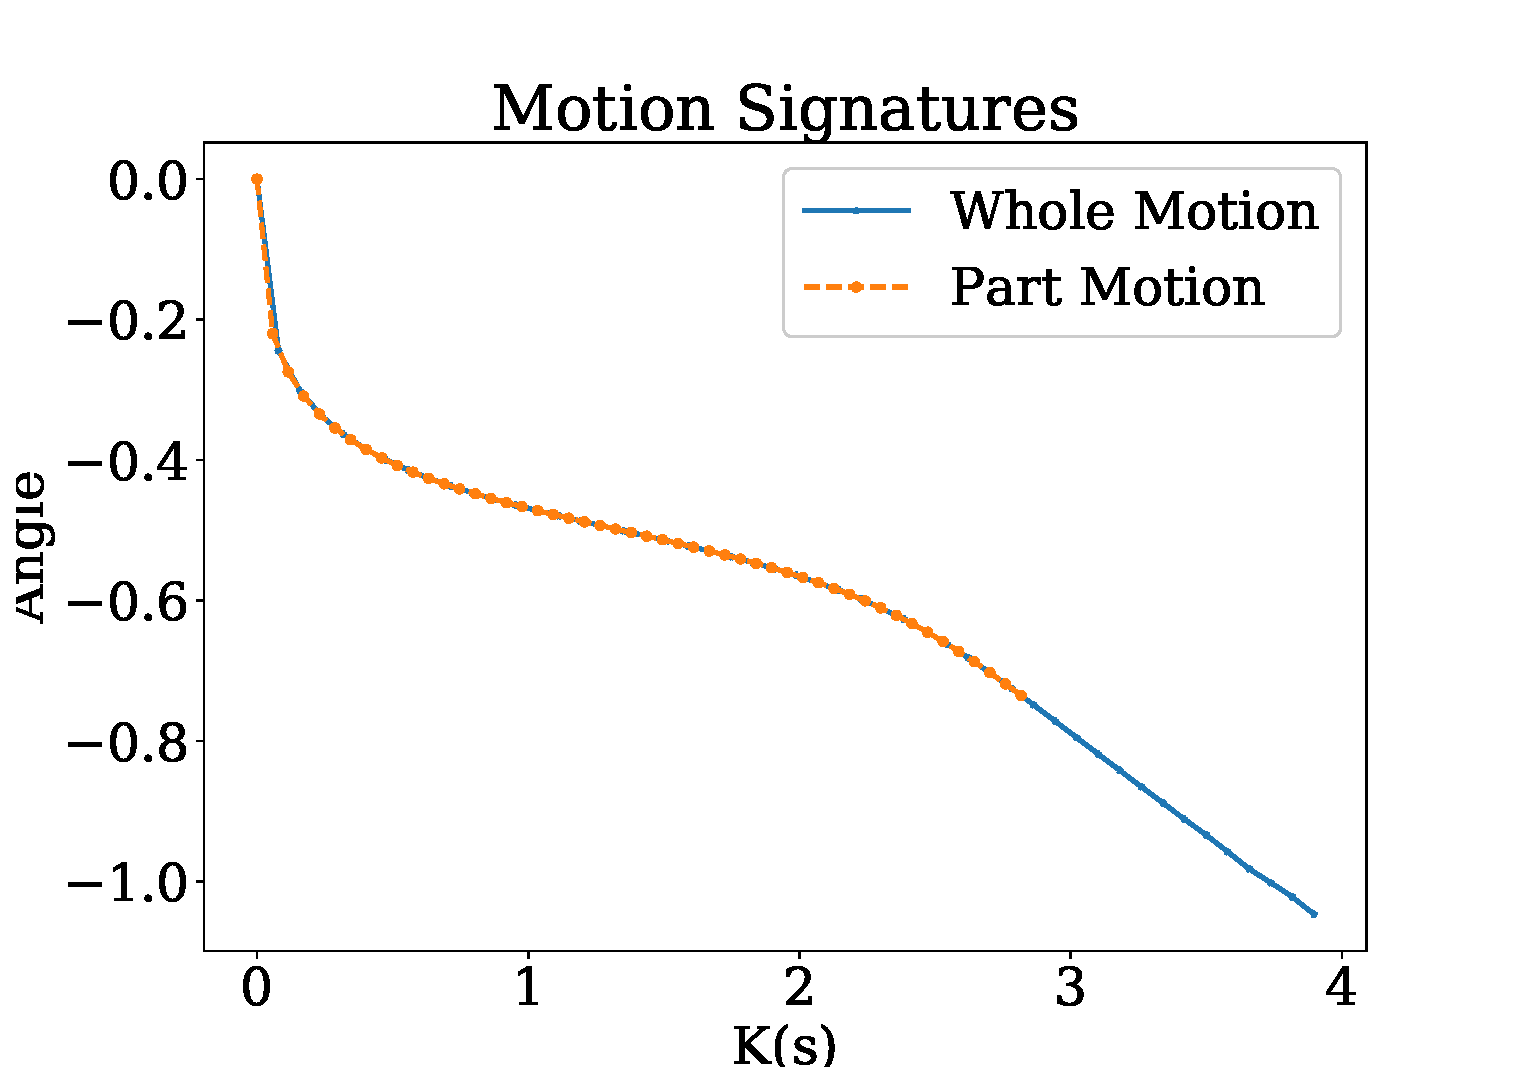
\includegraphics[width=260pt]{figure/fig_motion_signatures.eps}
  \caption{Motion Signatures of the trajectories shown in Fig.~\ref{wholePart}. The domain as well as range of motion signature is invariant to similarity transformation.}
\label{motionSignature}
\end{figure}

\begin{figure}
\centering
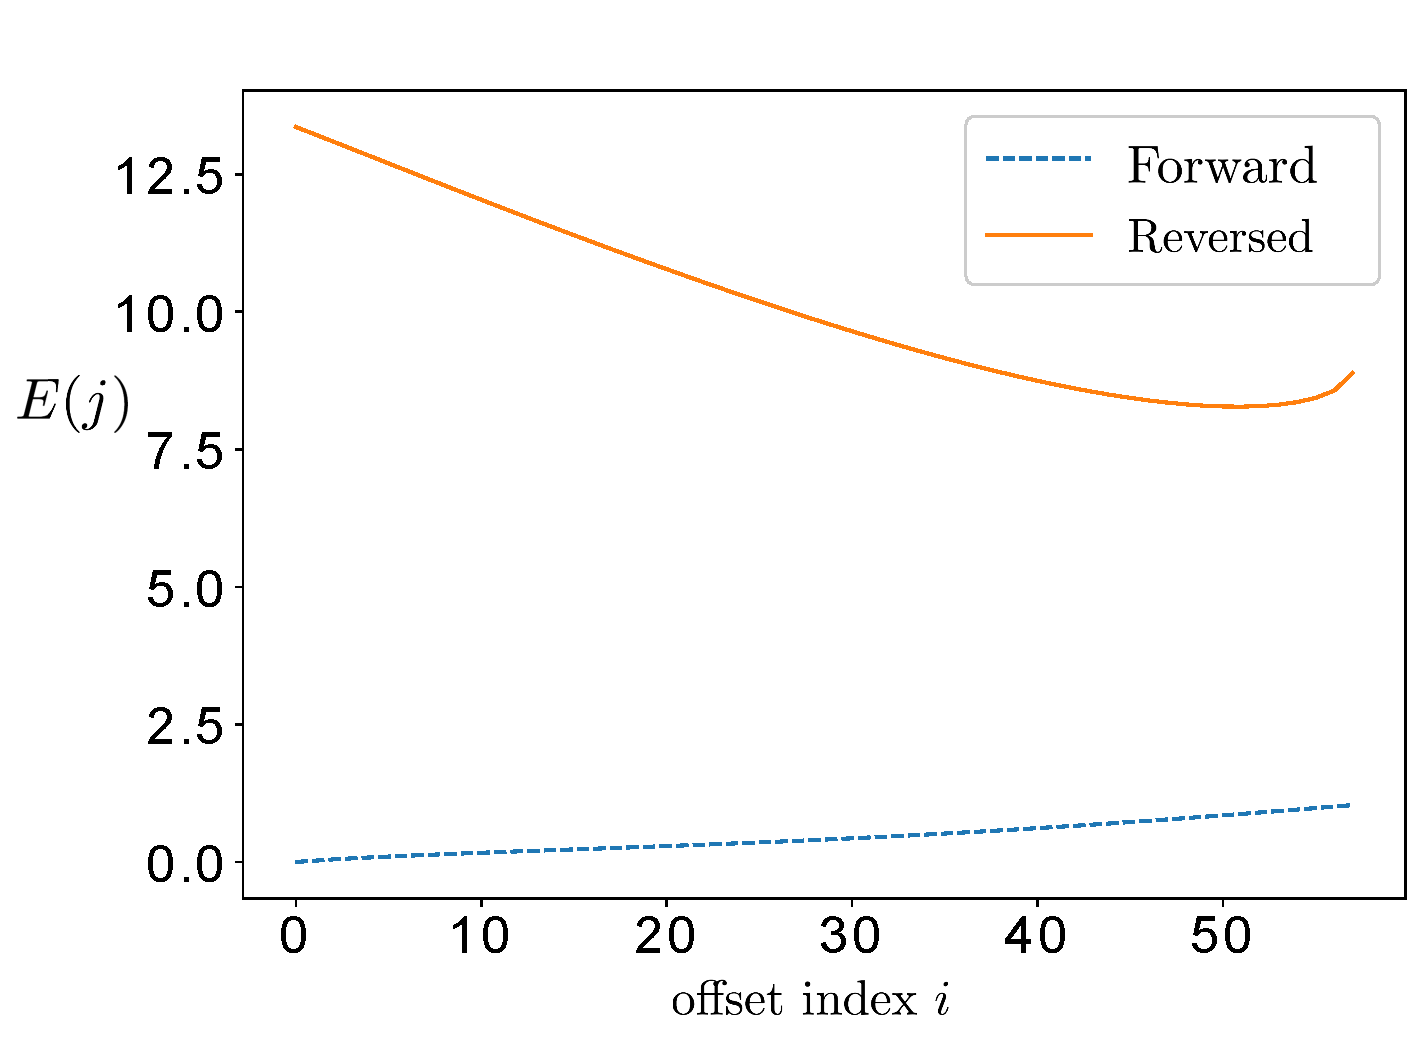
\includegraphics[width=240pt]{figure/fig_mcc.eps}
  \caption{Dissimilarity function of two motion signatures along both directions. It can be seen that the exact match is found at $j=0$, where the template is fully embedded inside the other motion.}
\label{mcc}
\end{figure}

\subsection{Objective Function for Synthesis}
The functions in Eq.~\req{nccEq} and ~\req{mccEq} presented in the sections \ref{sec_ncc} and \ref{sec_mcc} can be used as the error measure for path and motion synthesis of any planar linkage, where the objective is to find a linkage that produces a motion whose part or whole corresponds to the target motion (or path).
Thus, we can formulate the path synthesis problem as,
\begin{equation}\label{objectiveFunPath}
  \argminA_{\textbf{\emph{l}}, W_i} (1 - Cn_{max}(p, W_i)),
\end{equation}
where $\textbf{\emph{l}}$ is the vector of linkage parameters for particular planar linkage, $p$ is signature the of task path taken as the template and ${\{W_i\}}_{i=0}^{s}$ is the signature set of all $s$ coupler paths generated by the linkage corresponding to $\textbf{\emph{l}}$.
In case of four-bar, $\textbf{\emph{l}}: l_1, l_2, l_3, l_4, l_5$, where $l_i$ is link ratio of $i^{th}$ link shown in Fig~\ref{fourbar}.

Similarly, we can formulate motion synthesis problem as,
\begin{equation}\label{objectiveFunMotion}
  \argminA_{\textbf{\emph{l}}, W_i} (E_{min}(p, W_i)).
\end{equation}
Here, $E$ is the Dissimilarity function from Eq.~\req{mccEq} while $p$ and ${\{W_i\}}_{i=0}^{s}$ are motion signatures instead of path signatures.

\begin{figure}
\centering
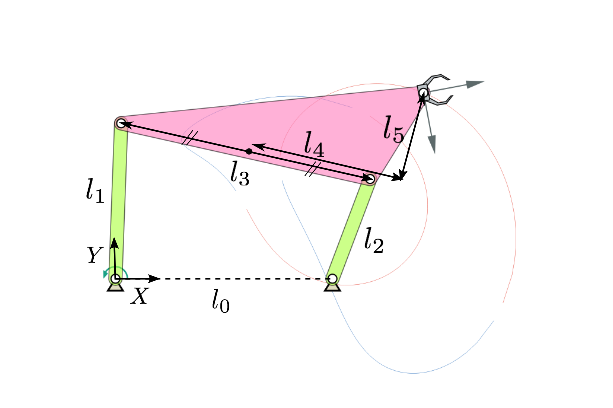
\includegraphics[width=270pt]{figure/fig_fourbar.eps}
  \caption{Parametric representation of four-bar linkage with all revolute joints. We set $l_0 = 1$ and one fixed joint at the origin of the global frame along with making the fixed length of four-bar parallel to the x-axis.}
\label{fourbar}
\end{figure}

Objective function evaluation step consists of calculation of coupler motion or path and finding its dissimilarity score.
It is important to note that representation obtained in Section~\ref{sec_sign} reduces the number of parameters in optimization.
This optimization problem can be solved using search methods which do not require gradient computation.
We can employ global optimization methods such as differential evolution at the start, and local optimization approach, such as Powell's method towards the end for faster convergence\cite{ullah1997}.

Considering the highly nonlinear nature of the problem, finding a good initial guess proves to be daunting. In addition, generating a large set of solutions requires a diverse and large number of good initial guesses.
Thus, we exploit machine learning techniques to create a database for finding many good initial guesses or the solution itself.
Section~\ref{sec_db_ae} presents the details of this approach.


\section{Sensitivity Analysis of Signatures}\label{sec_SA}
Due to the complex relationship between parameter space and generated motion, small changes in linkage parameters can produce large and discontinuous structural changes in the generated motions.
For example, a small change in crank length ($l_1$) can open a previously closed coupler path.
Most of the methods based on Fourier descriptors cannot capture the continuity at such singular locations, which adversely affect the optimization process.
In contrast to this behavior, the signatures derived in Sec.~\ref{sec_sign} have a smooth transition at these singular locations due to shape similarity between closed and just opened curve or motion.

To illustrate this via an example, we perform sensitivity analysis in the vicinity of a singularity as follows:
A four-bar with link ratios ($l_1:0.55$, $l_2:1$, $l_3:1.5$, $l_4:1$, $l_5:1$) is subjected to gradual change in parameters $l_1$ and $l_3$ by the amount (-0.2, 0.2) in steps of 0.01.
The link ratios are chosen such that, small changes in some parameters lead to the topological change in the coupler curve.
Error function between motions of new and initial four-bar are calculated using Eq.~\req{objectiveFunMotion}. Figure~\ref{saCouplerCurves} shows coupler motion of some of the four-bars, while Fig.~\ref{saMotionSignatures} depicts their motion signatures. Please note that these two figures show the effect of changing only one parameter $l_1$.
It can be seen from Fig.~\ref{saCouplerCurves} that there exists a discontinuity in the topology of coupler curves even though their shapes have a continuous shift.
Our method captures this continuity, which is shown by error function evaluations depicted in Fig.~\ref{saErrorFunction}, where it is visible that surface is well behaved in the singularity region. This error function accounts for changes to both the parameters $l_1$ and $l_3$.

\begin{figure}
\centering
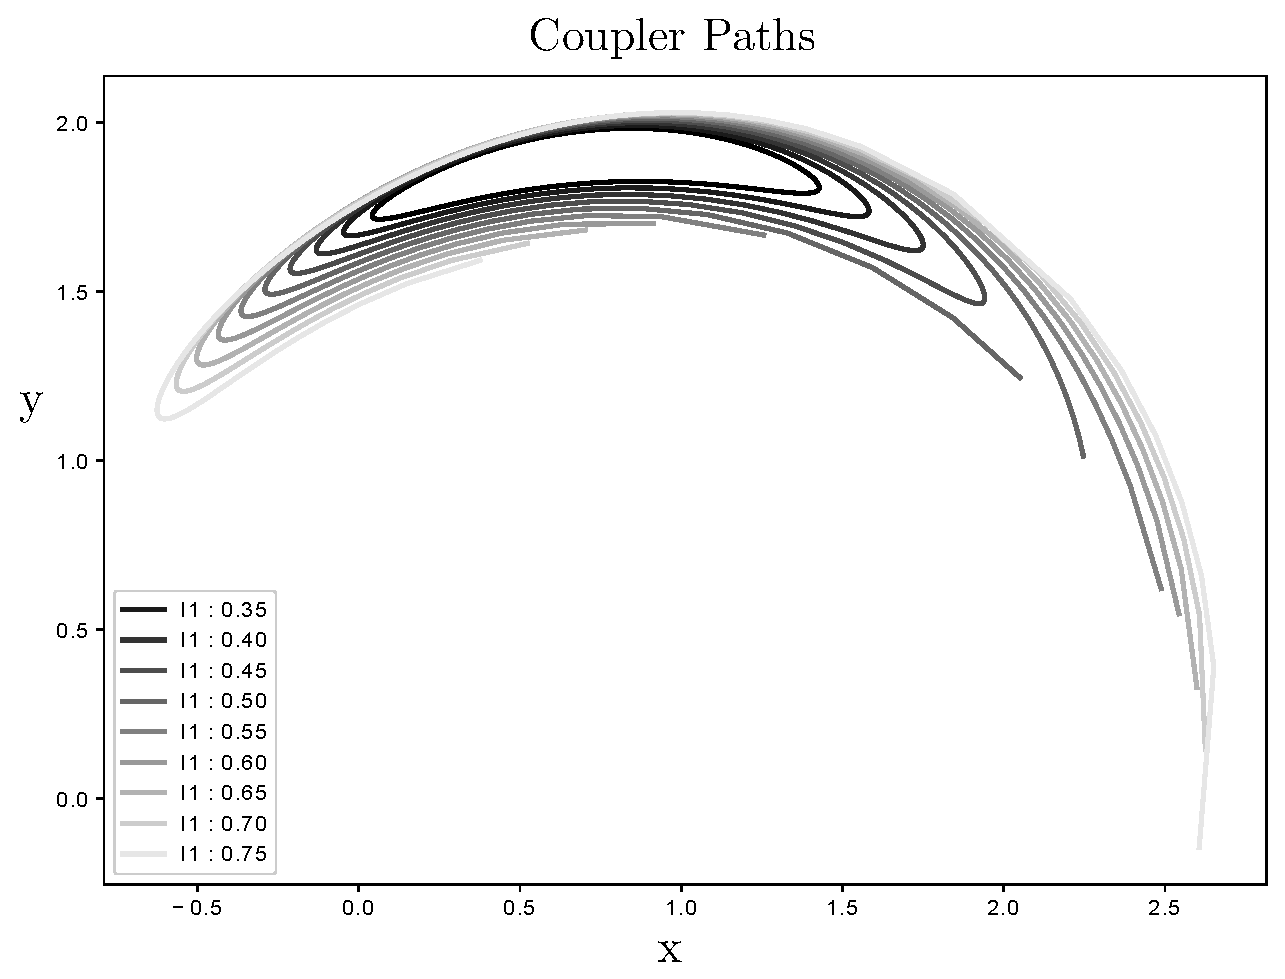
\includegraphics[width=240pt]{figure/fig_sa_coupler_curves.eps}
  \caption{Coupler Motions of the four-bar linkage with variation of parameters $l_1$ and $l_2$. It can be seen that motion topology changes from close-loop Grashof to open loop Triple-Rocker.}
\label{saCouplerCurves}
\end{figure}

\begin{figure}
\centering
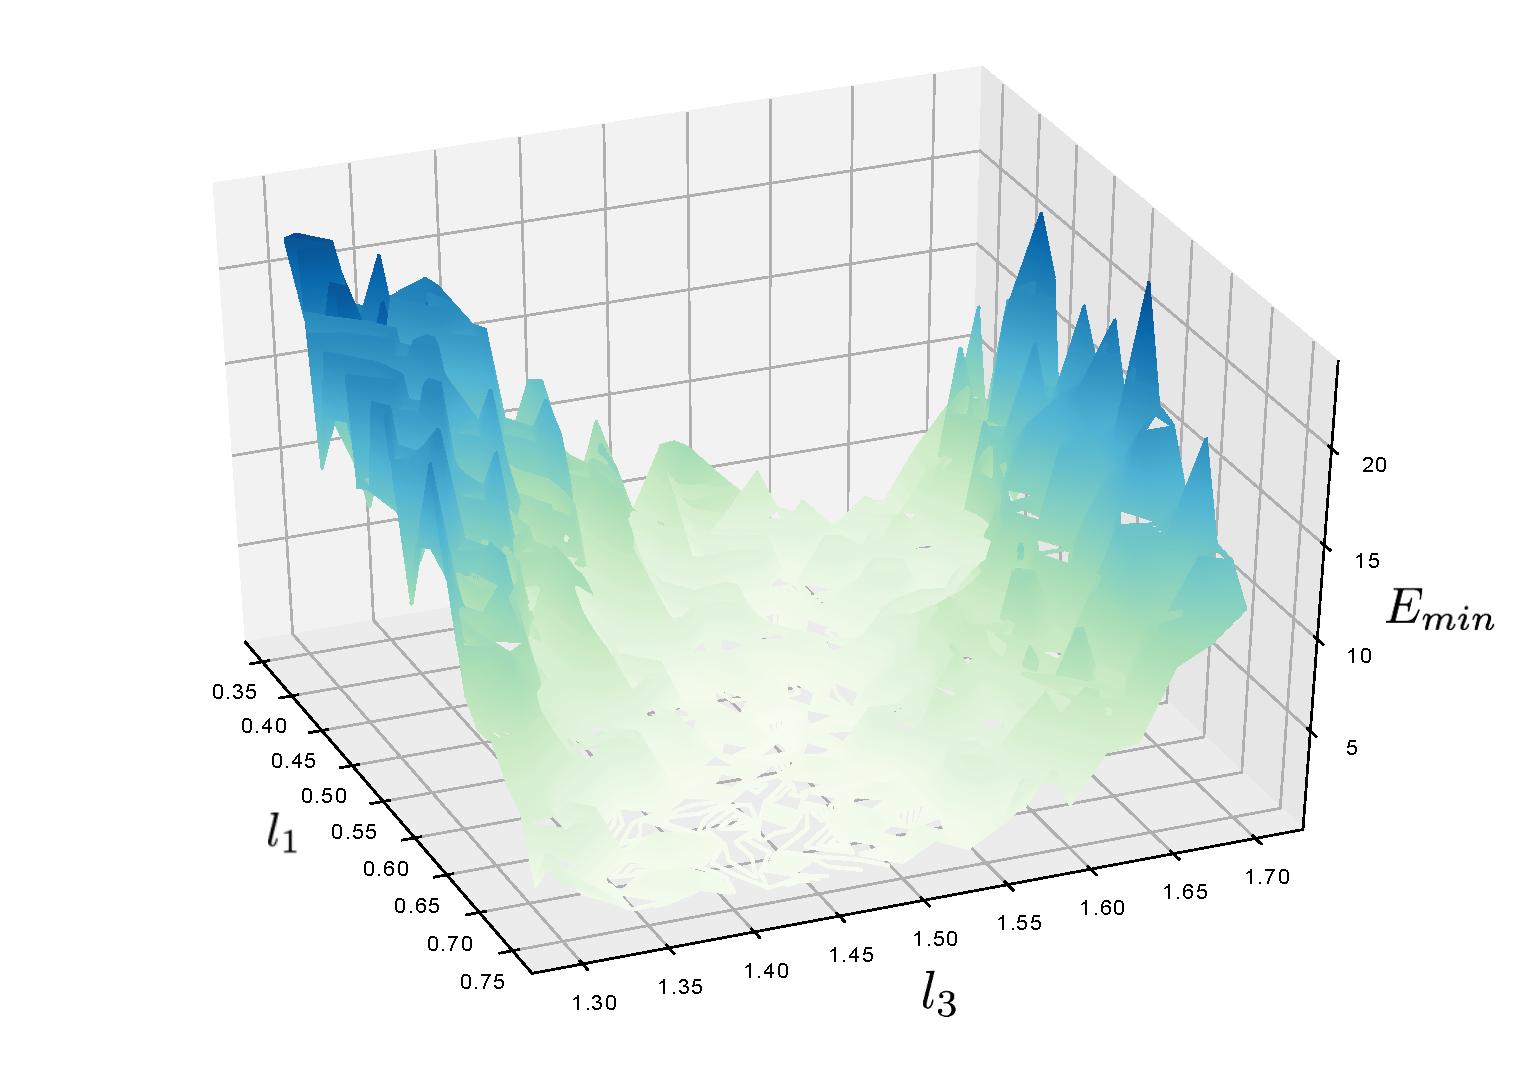
\includegraphics[width=240pt]{figure/fig_sa_distance_function.eps}
  \caption{Distance ($E_{min}$) from Eq.~\req{mccEq} as the parameters $l_1$ and $l_3$ are varied. Although open loop breaks at $l_1$:0.55, $l_3$:1.5, there are no spikes of error function in the region near singularity, as the shape is very similar between the two topologies.}
\label{saErrorFunction}
\end{figure}

\begin{figure}
\centering
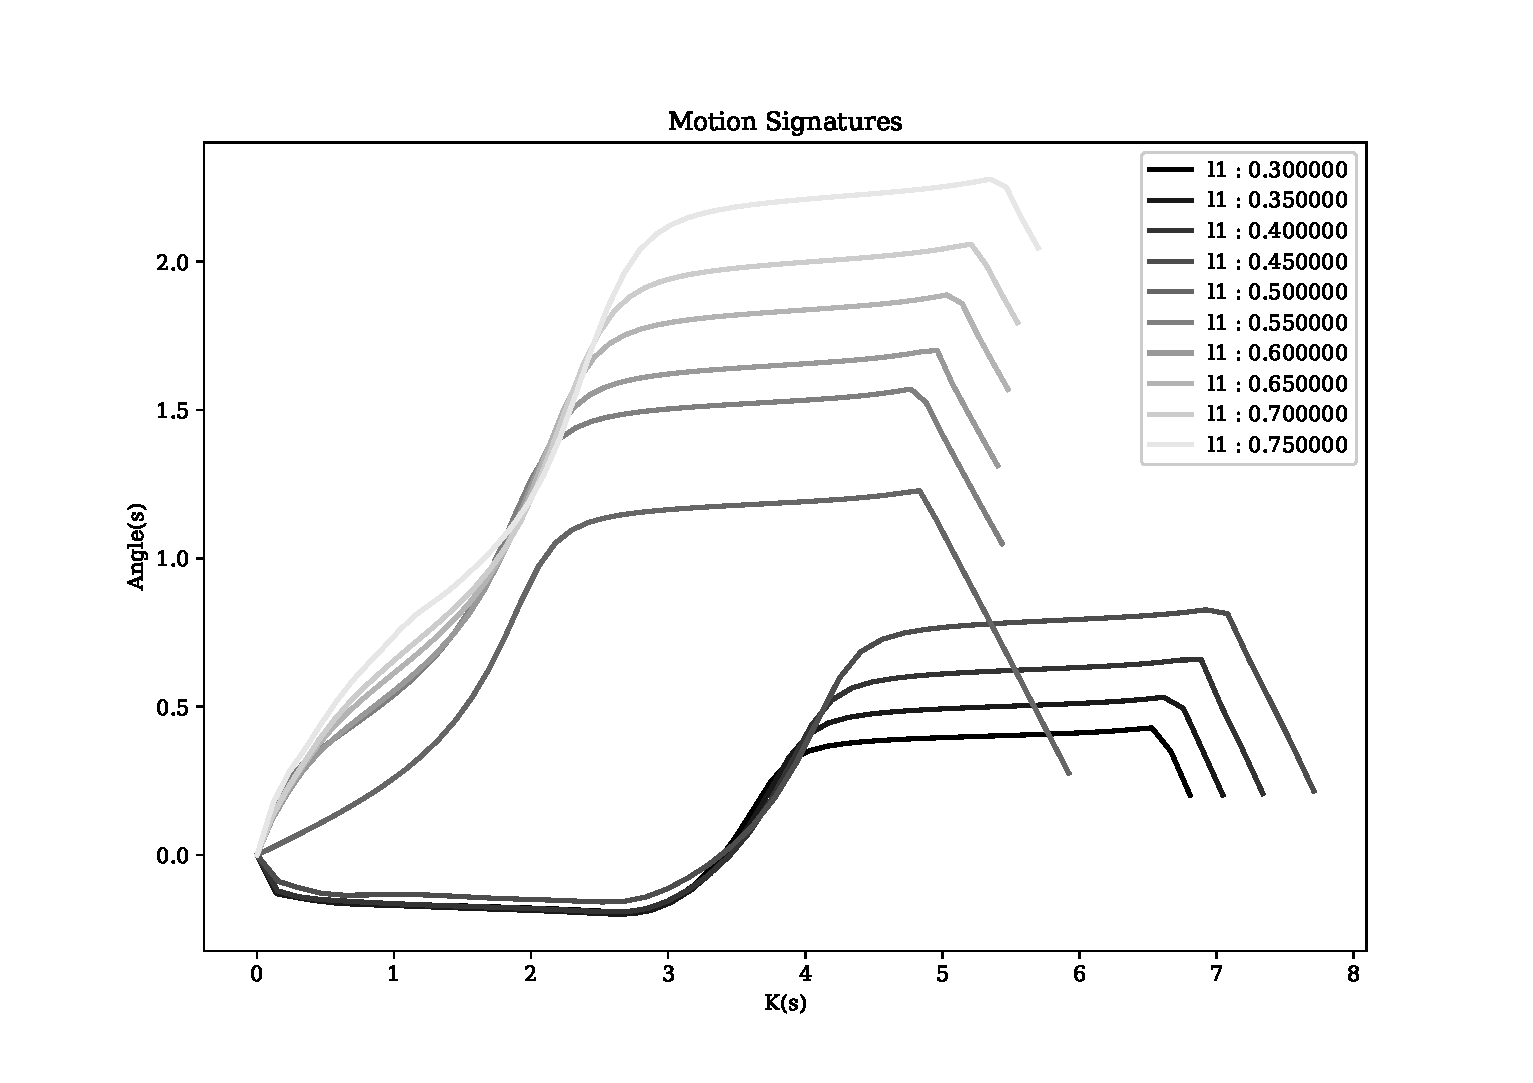
\includegraphics[width=240pt]{figure/fig_sa_motion_signatures.eps}
  \caption{Motion signatures obtained by steps given in~\ref{sec_sign}. Although topology difference is even more evident in this representation, it also signifies the similarity pattern between them.}
\label{saMotionSignatures}
\end{figure}

\section{Clustered Database of Planar Linkages}\label{sec_db_ae}

Having an invariant representation facilitating partial matching greatly reduces data required to sample all possible types of shapes of coupler motion.
We have built a database of planar four-bar linkages with revolute joints as an example, but the approach is the same for any planar motion generating mechanism.
We generate this database comprising of $40,000$ linkages while taking following aspects into consideration:
\begin{enumerate}
  \item Sampling should maximize the uniformity of its distribution over the space of four-bar coupler motions.
  \item Data generation should be parallelized.
  \item It should be scalable to higher-order linkages.
\end{enumerate}
Figure~\ref{fourbar} represents parametric representation of four-bar linkage with parameters ($l_1,l_2,l_3,l_4,l_5$).
As mapping between four-bar linkage parameter space and coupler motion space is highly nonlinear, uniform distribution over linkage parameter space does not necessarily mean uniform sampling over coupler motion space.
Thus, an efficient approach would be to sample more in the regions where sensitivity is maximum.
We have observed that whenever the link ratios of four-bar linkage are close to 1, the sensitivity of shape of a coupler motion is higher than otherwise.
Thus, we have chosen Log Normal probability distribution ($\mu = 0,\sigma = 0.6 $) for selecting the link ratios : $(l_1, l_2, l_3)$ as shown in Fig.~\ref{logNormal}, and Normal Distribution ($\mu = 0,\sigma = 2 $) for $(l_4, l_5)$.

\begin{figure}
\centering
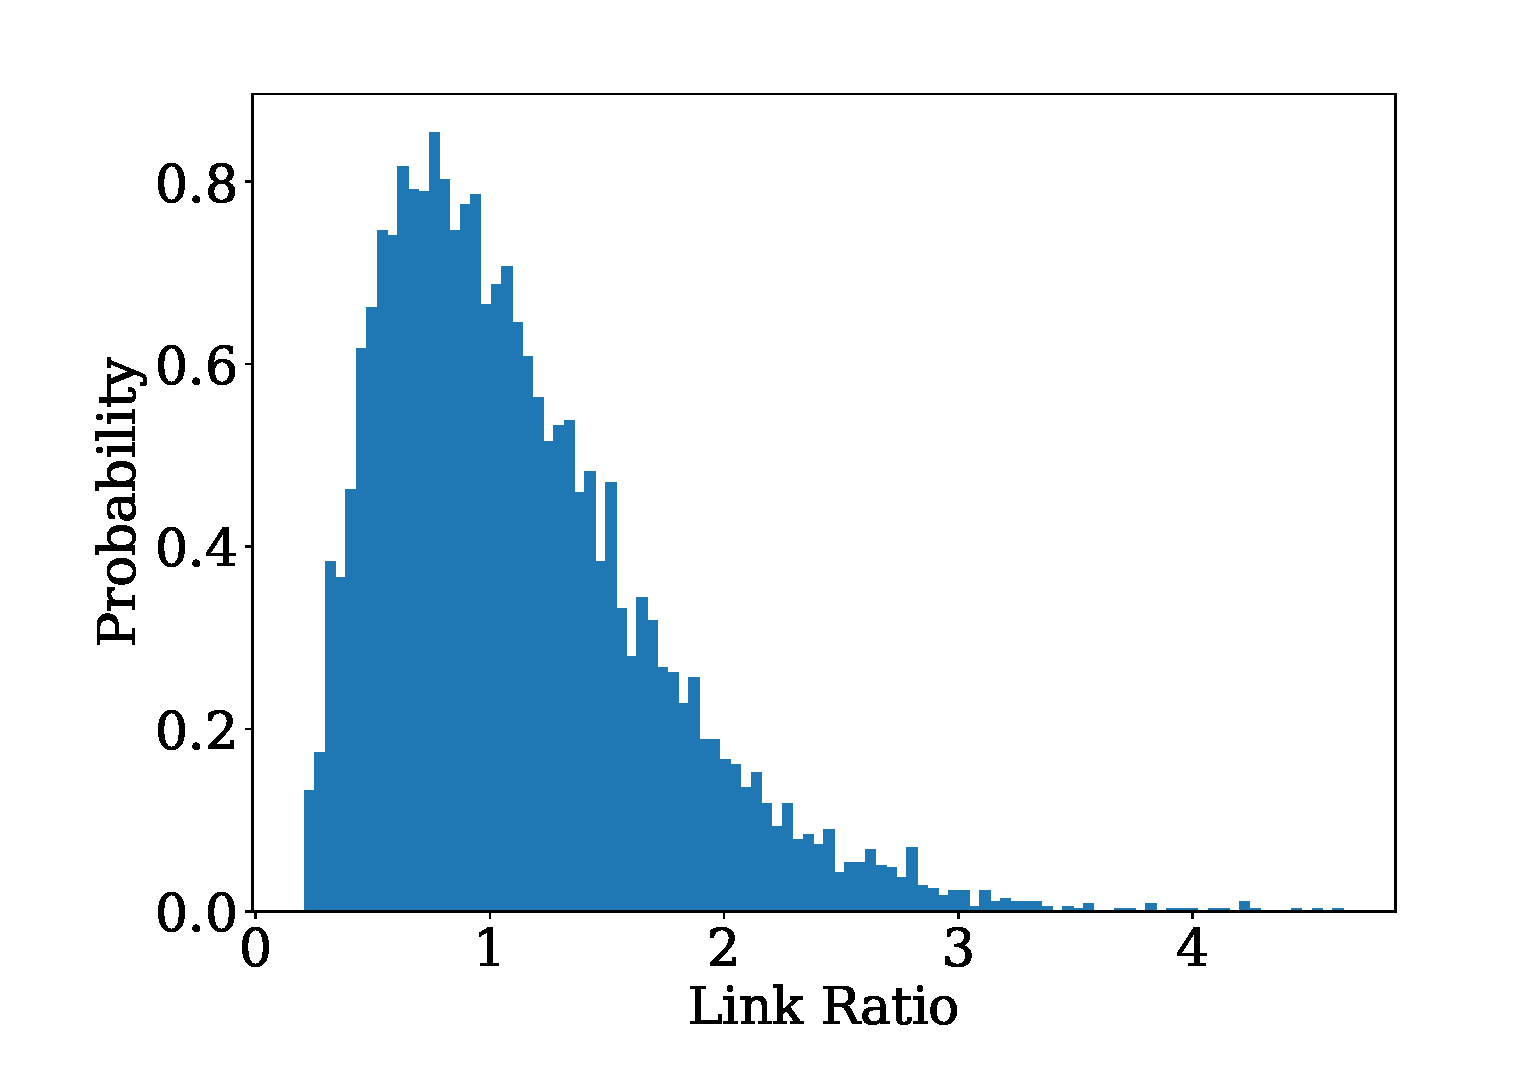
\includegraphics[width=240pt]{figure/fig_logNormal.eps}
  \caption{Probability Distribution function used in random sampling for parameters $l_1$, $l_2$ and $l_3$.}
\label{logNormal}
\end{figure}

We use machine learning techniques such as clustering and data-compression using auto-encoder neural networks to come up with good initial guesses for local optimization.
First, We cluster the database using a hierarchical clustering algorithm.
Then, we find a representative data point in each cluster called cluster centers and form their set.
This set of cluster centers represent a diverse group of linkages.
When a query is raised in the database, the first step is to search for neighbors in the set of cluster centers.
This often yields a diverse set of neighbors and is used as the set of independent initial guesses for local optimization.

\subsection{Dimensionality Reduction using Auto-Encoders}
Each data point in the database consists of a discrete signature, which is kept to be of 100 float digits.
In order to have efficient query operations, we perform hierarchical Clustering; a method that summarizes and creates a hierarchy in the database.
Clustering in higher dimensions suffers from \emph{Curse of Dimensionality}\cite{marimont1979}, thus we first perform dimensionality reduction using Auto-encoder Neural Networks.
Auto-encoder is a powerful mapping model, which learns to encode the input data in very compact representation and can reconstruct the input with minimal error; performing much better than Principal Component Analysis\cite{hinton2006}.
This nonlinear mapping by auto-encoder can greatly improve the representation of data for clustering~\cite{song2013}.
Figure~\ref{autoEncoder} shows a Neural Network architecture similar to the one we designed for the task.
Our architecture consists of 100 neurons in the input and output layer, while the five hidden layers have (80, 50, 10, 50, 80) neurons respectively.
Each neuron in the hidden layer is activated by Rectified Linear Unit (\emph{ReLU}) activation function.
In $i^{th}$ hidden layer, $d^{(i-1)}$ dimensional vector output of the previous layer $h_(i-1)$ is fed as input to produce $d^{(i)}$ dimensional output $h_i$.
Input-output relationship of a layer is given by,

\begin{eqnarray}\label{nnlayer}
  h_i = ReLU(W_{i}h_{i-1} + b_{i}), \\
  ReLU(x) = max(0, x),
\end{eqnarray}
where $W_i$ is weight matrix with dimensions $(d^{i}, d^{(i-1)})$ and $b_i$ is $d^{(i)}$ dimensional bias vector of $i^{th}$ layer, which are computed in the process of training.
Auto-encoders are trained to reconstruct the input.
In this way, each layer encodes the input, which is sufficient for the next layers to reconstruct the output.
The objective of training is to find out the set of weights and biases that minimizes the error loss given by,

\begin{equation}\label{nnloss}
  \argminA_{W, b} \sum_{i=0}^{N} || X_i - \tilde{X}_i ||^2,
\end{equation}
where $X_i$ is input, $\tilde{X}_i$ is reconstructed output and N is number of training examples.


Once a network is trained, the output of the bottle-neck layer $(h_{ib})$ represents the compressed feature space ($Z$).
As bottleneck layer has 10 neurons and input is a 100-dimensional vector, it is evident that information is compressed by a factor of 10, while achieving $95\%$ reconstruction accuracy as the result of training.
Standard clustering algorithms are performed on this latent\footnote{compressed output of bottleneck layer.} space for better clustering\cite{song2013}.
We use Agglomerative Clustering, a method of hierarchical clustering, which is an approach to partitioning clustering for identifying groups in the dataset.
\emph{Ward}\cite{ward1963} criterion is used for clustering, which minimizes the variance of the clusters being merged.
The distance metric used for clustering is the Euclidean distance in the latent space.
Although the more accurate distance metric is the distance function discussed in the section~\ref{sec_distanceMetric}, it is very expensive to calculate it for the entire database.
Signatures with ${O}(m)$ points take ${O}(m\log{}m)$ time for each comparison and there are ${O}(N^2)$ number of comparisons to be made for the database of $N$ points.

Now, when the user raises a query, we use the distance function from the section~\ref{sec_distanceMetric} for finding $k$ nearest neighbors among $1500$ cluster centers.
If a cluster center is not sufficiently close, we descend into its corresponding cluster to find the closest data point.
Motion with highest similarity score is returned along with its corresponding linkage parameters.
If required, the parameters are fine-tuned to match the query using local optimization methods.
Computationally, on a 2.4 GHz Core i5 MacBook Pro with 8 GB memory, every query takes 23 seconds on average to find the sorted list of nearest neighbors among cluster centers.

\begin{figure}
\centering
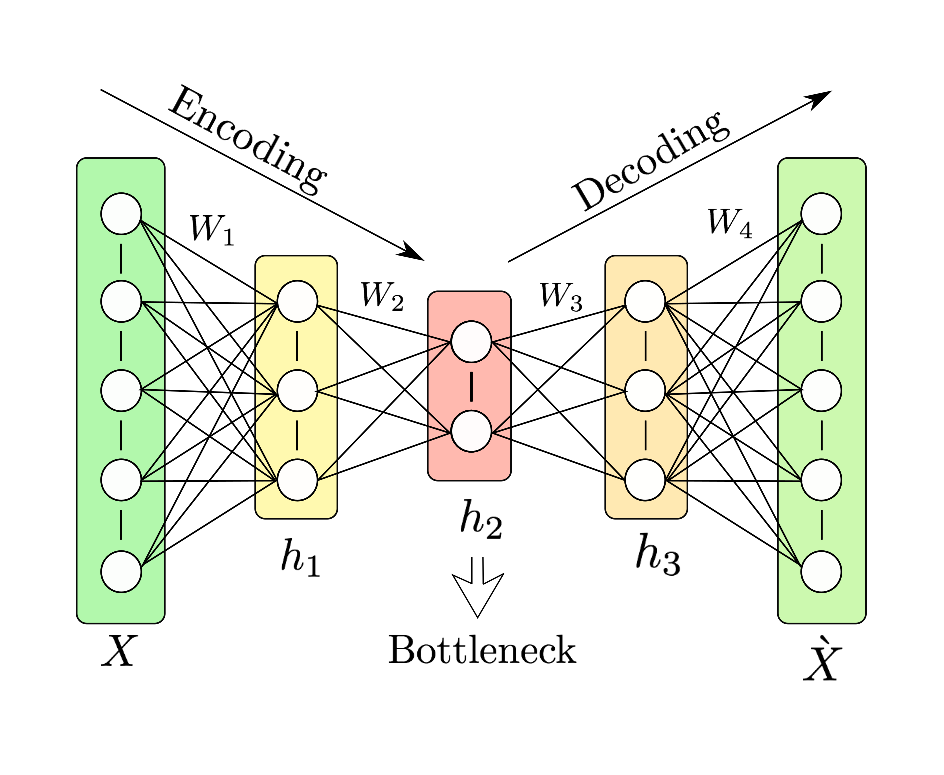
\includegraphics[width=270pt]{figure/fig_auto_encoder.eps}
  \caption{A small-scale version of the Auto-Encoder. This network takes 5-dimensional input in the input layer. At each encoder layer, the input is compressed into a vector of lower dimensions, the lowest at the bottleneck layer.}
\label{autoEncoder}
\end{figure}


\section{Case Studies}\label{sec_example}
This section presents two case studies presenting the effectiveness of our approach for path and motion synthesis applications.
\subsection{Path Generation}
In the design phase of a rehabilitation device that assists people to stand from sitting position, it is required to generate linkages that can execute a sit-to-stand (STS) trajectory of the hip joint as shown in Fig.~\ref{ex1_path}.
Table~\ref{hipPathTab} presents the discretized path data.
As our approach requires parametric representation of path, we first fit a cubic B-Spline with cord length parametrization through path data points to generate parametric curve shown in Fig.~\ref{ex1_path}.
We compute its path signature by the steps mentioned in Algorithm ~\ref{alg_signature} and raise the query for nearest neighbors among 1500 cluster centers of our database.
The distance metric for finding neighbors among cluster centers is $1-Cn_{max}$ in Eq.~\req{objectiveFunPath}.
Table~\ref{ex1_knnLinkageData} tabulates the link ratios corresponding to obtained nine nearest neighbors.
Next step is to compute actual parameters according to position, scale, and orientation of the path.
It is done by comparing analogous points found by the offset index $j$ in Eq.~\ref{nccEq}.
Figure ~\ref{ex1_solns} shows the first eight four-bar mechanisms corresponding to nearest signatures to path signature of input.
It can be clearly seen that these linkages generate highly accurate paths for the sit to stand activity.
It is important to note that every solution is a result of partial matching of coupler paths, and otherwise would be very hard to search using other atlas-based approaches that only have the whole-to-whole matching facility.

\begin{table}
\caption{Case Study 1 : Path Data}
\centering
\label{hipPathTab}
\begin{tabular}{cccccc}
\hline
Point & x & y & Point & x & y \\
\hline
1 & -7.81 & -9.65 & 10 & 0.28 & -1.31 \\
2 & -6.42 & -9.81 & 11 & 0.64 & 1.07 \\
3 & -5.14 & -9.62 & 12 & 0.98 & 2.73 \\
4 & -3.72 & -8.99 & 13 & 1.47 & 4.30 \\
5 & -2.62 & -8.14 & 14 & 2.73 & 6.58 \\
6 & -1.75 & -7.13 & 15 & 3.46 & 7.41 \\
7 & -0.91 & -5.67 & 16 & 4.07 & 7.95 \\
8 & -0.32 & -4.10 & 17 & 4.70 & 8.41 \\
9 & -0.02 & -2.92 & 18 & 5.32 & 8.76 \\
\end{tabular}
\end{table}

\begin{table}
\caption{Linkage Parameters of Nine Nearest Neighbor Paths}
\centering
\label{ex1_knnLinkageData}
\begin{tabular}{ccccccc}
\hline
  linkage & $l_1$ & $l_2$ & $l_3$ & $l_4$ & $l_5$ & $1 - Cn_{max}$ \\
\hline
 1 & 0.79 & 2.78 & 1.70 & 1.35 & -0.71 & 0.0011 \\
 2 & 1.59 & 1.28 & 0.96 & -1.74 & -1.13 & 0.0015\\
 3 & 0.99 & 0.71 & 1.66 & -1.07 & -0.85 & 0.0016\\
 4 & 0.51 & 0.48 & 1.11 & -0.02 & -0.15 & 0.0017\\
 5 & 0.93 & 0.75 & 2.18 & -1.65 & 0.96 & 0.0018 \\
 6 & 1.29 & 1.98 & 1.02 & -1.83 & -1.33 & 0.0019\\
 7 & 0.63 & 1.42 & 1.03 & -1.90 & -0.38 & 0.0020\\
 8 & 0.66 & 0.85 & 0.84 & -1.40 & -0.13 & 0.0021\\
 9 & 1.81 & 0.55 & 1.08 & 0.14 & -0.04 & 0.0022
\end{tabular}
\end{table}

\begin{figure}
\centering
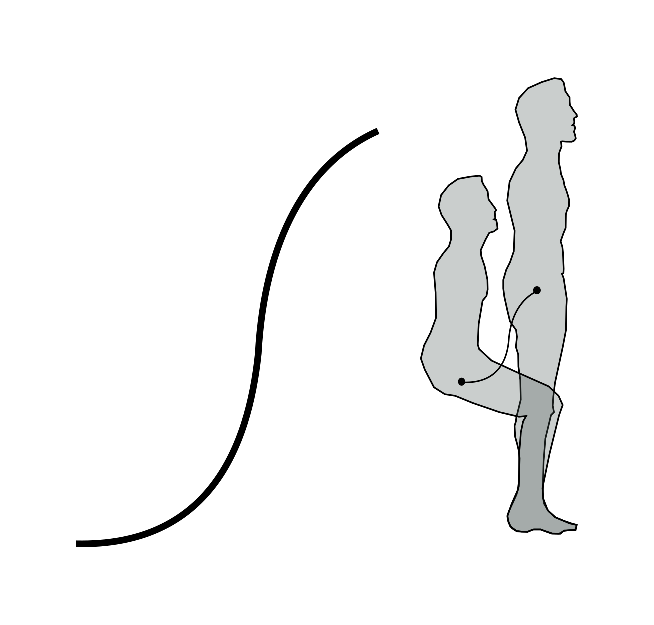
\includegraphics[width=240pt]{figure/path_solutions/hip_path.eps}
  \caption{Case Study 1: Path traced by hip joint during Sit-to-Stand Motion.}
\label{ex1_path}
\end{figure}

\begin{figure}
\begin{tabular}{cc}
  1)\putindeepbox[7pt]{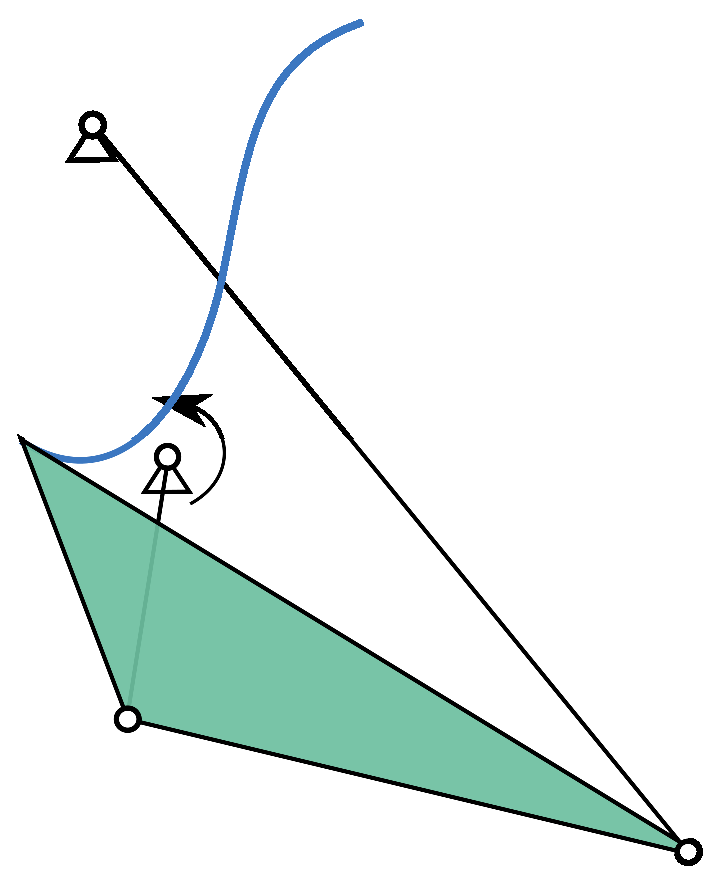
\includegraphics[width=100pt]{figure/path_solutions/path_sol1.eps}}
    & 2)\putindeepbox[7pt]{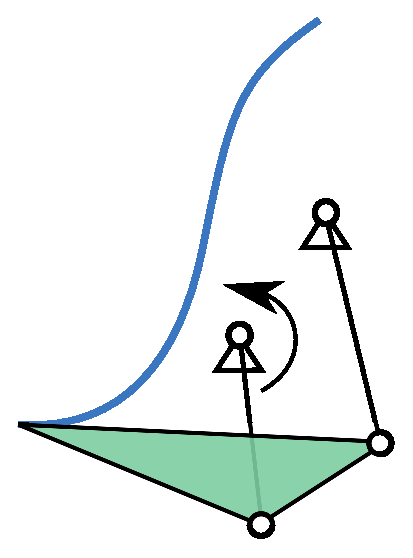
\includegraphics[width=60pt]{figure/path_solutions/path_sol2.eps}} \\
  3)\putindeepbox[7pt]{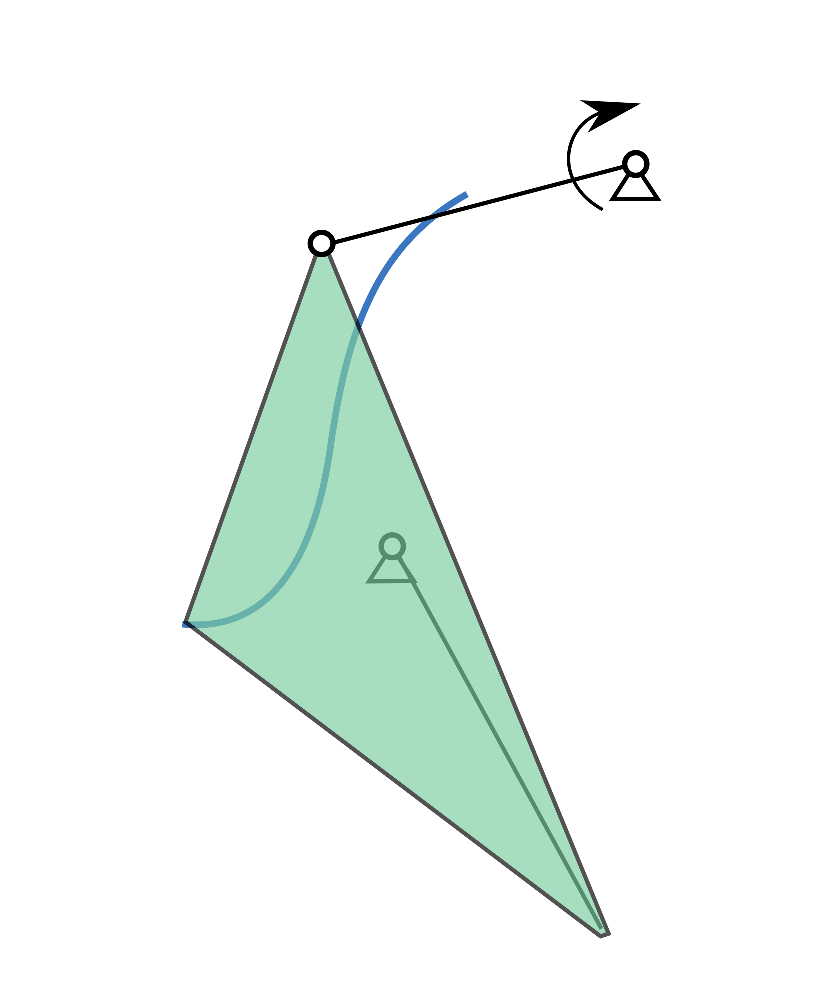
\includegraphics[width=100pt]{figure/path_solutions/path_sol3.eps}}
    & 4)\putindeepbox[7pt]{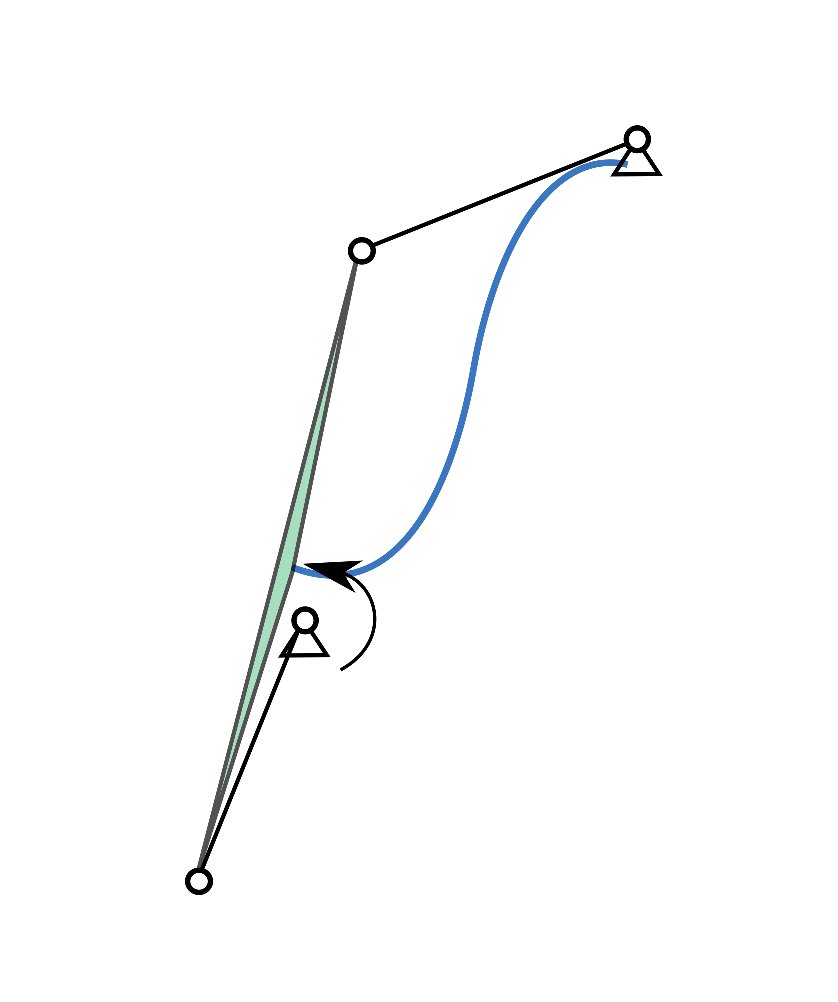
\includegraphics[width=100pt]{figure/path_solutions/path_sol4.eps}}\\
  5)\putindeepbox[7pt]{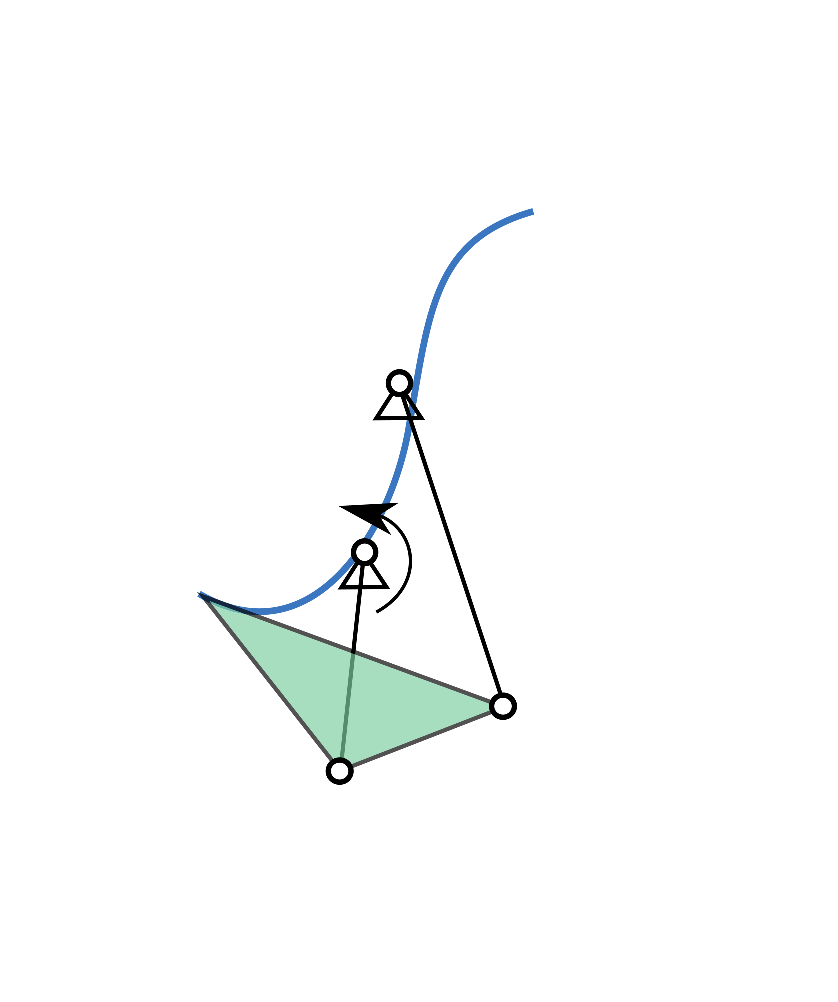
\includegraphics[width=100pt]{figure/path_solutions/path_sol5.eps}}
    & 6)\putindeepbox[7pt]{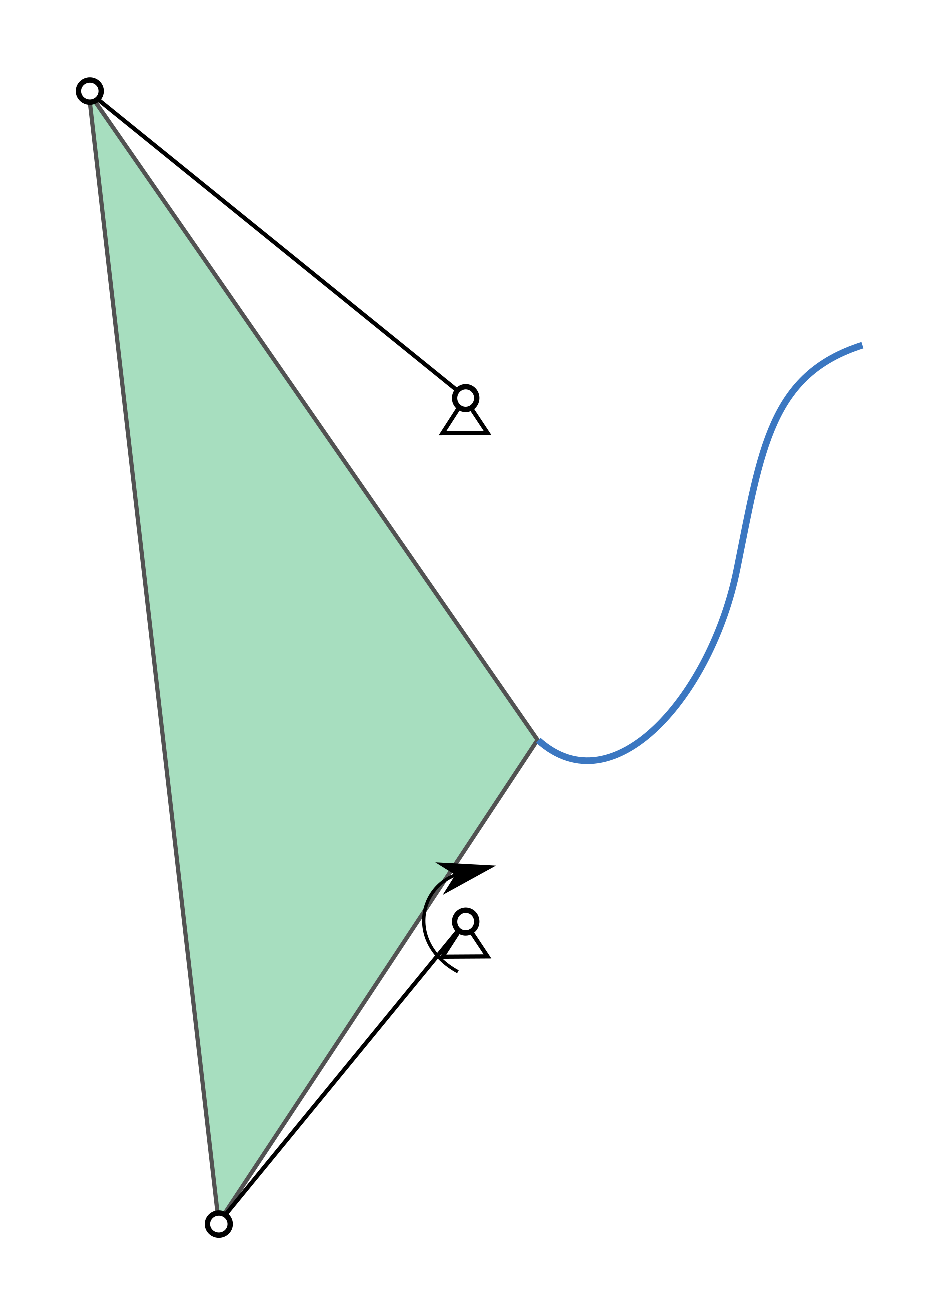
\includegraphics[width=100pt]{figure/path_solutions/path_sol6.eps}} \\
  7)\putindeepbox[7pt]{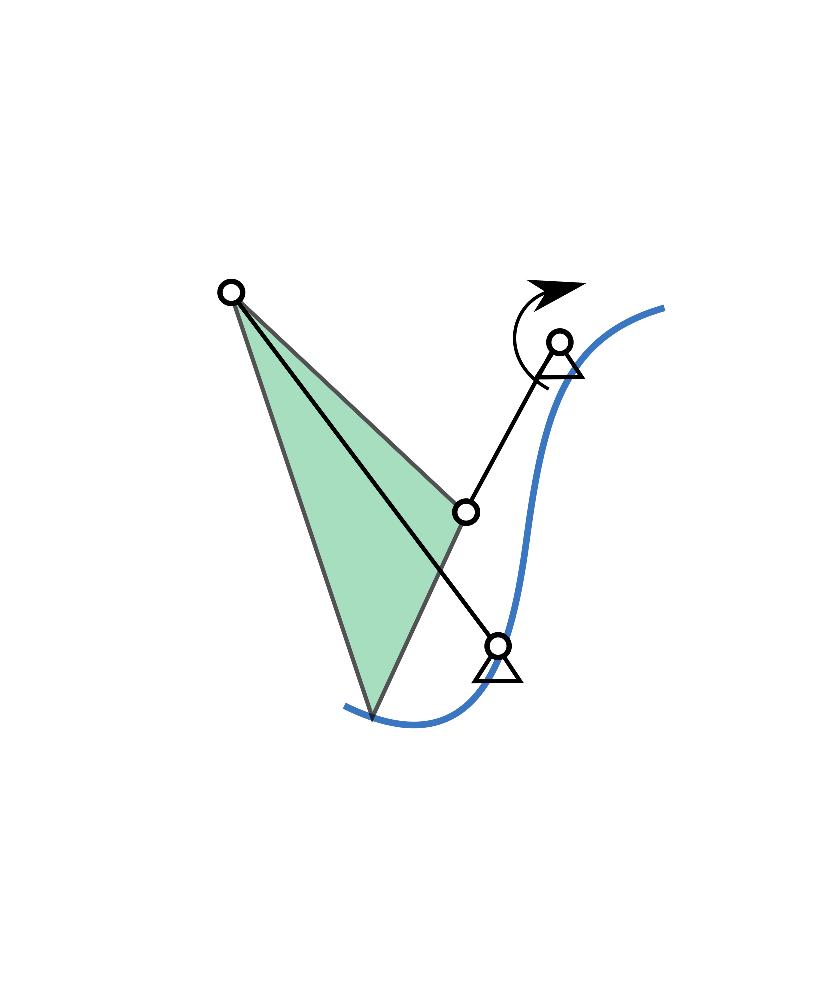
\includegraphics[width=100pt]{figure/path_solutions/path_sol7.eps}}
    & 8)\putindeepbox[7pt]{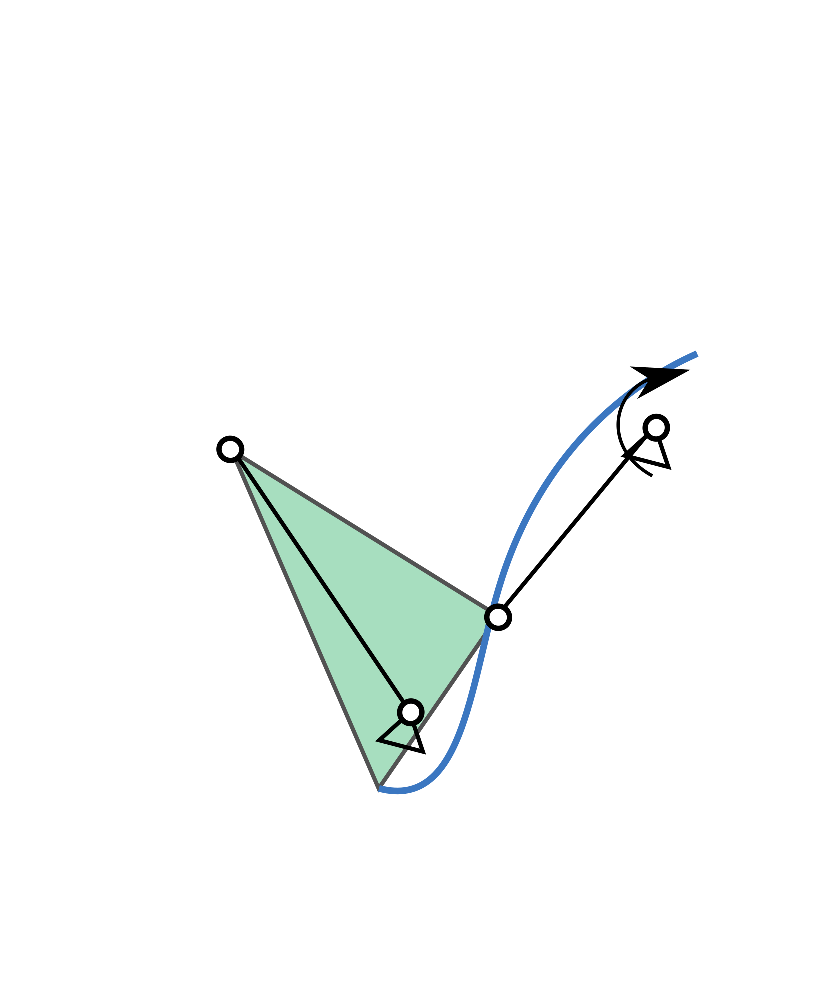
\includegraphics[width=100pt]{figure/path_solutions/path_sol8.eps}}\\
\end{tabular}
\caption{First eight linkages in the table~\ref{ex1_knnLinkageData} and their resultant coupler paths.}
\label{ex1_solns}
\end{figure}

\subsection{Motion Generation}\label{subsec_motiongen}

\begin{figure}
\centering
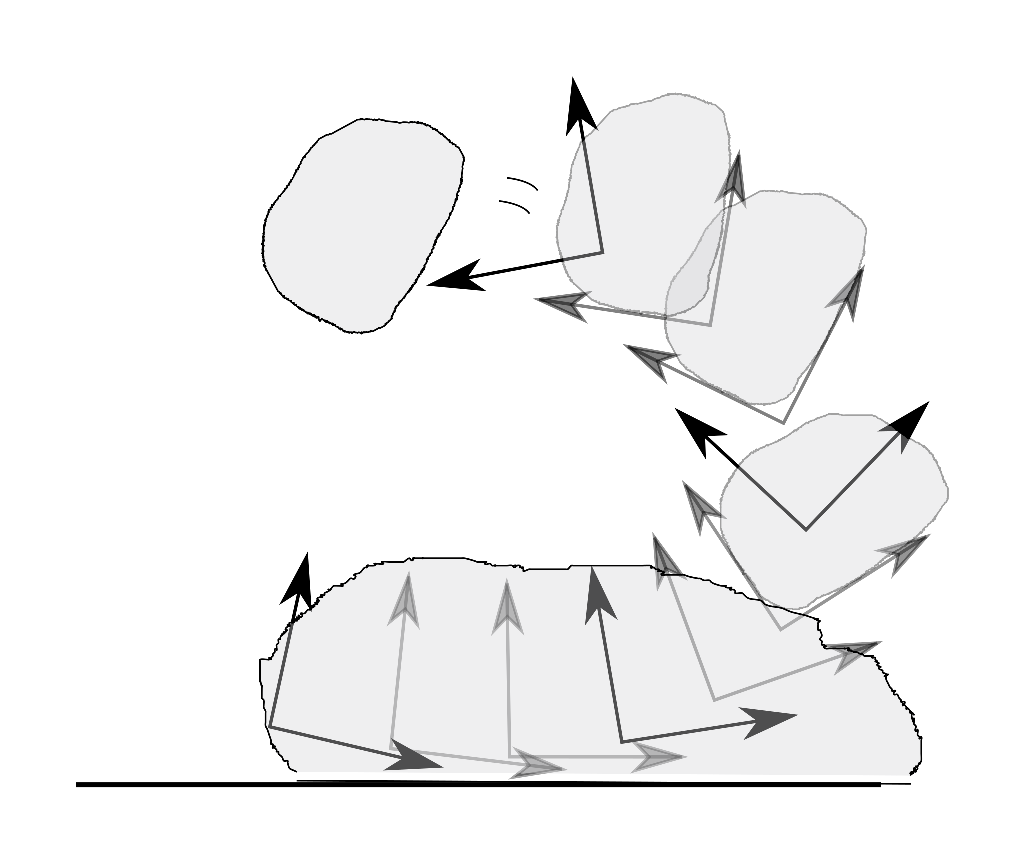
\includegraphics[width=240pt]{figure/fig_motion_query.eps}
  \caption{Case Study 2: User specified motion necessary for the snow shoveling task.}
\label{motionQuery}
\end{figure}

\begin{figure}
\centering
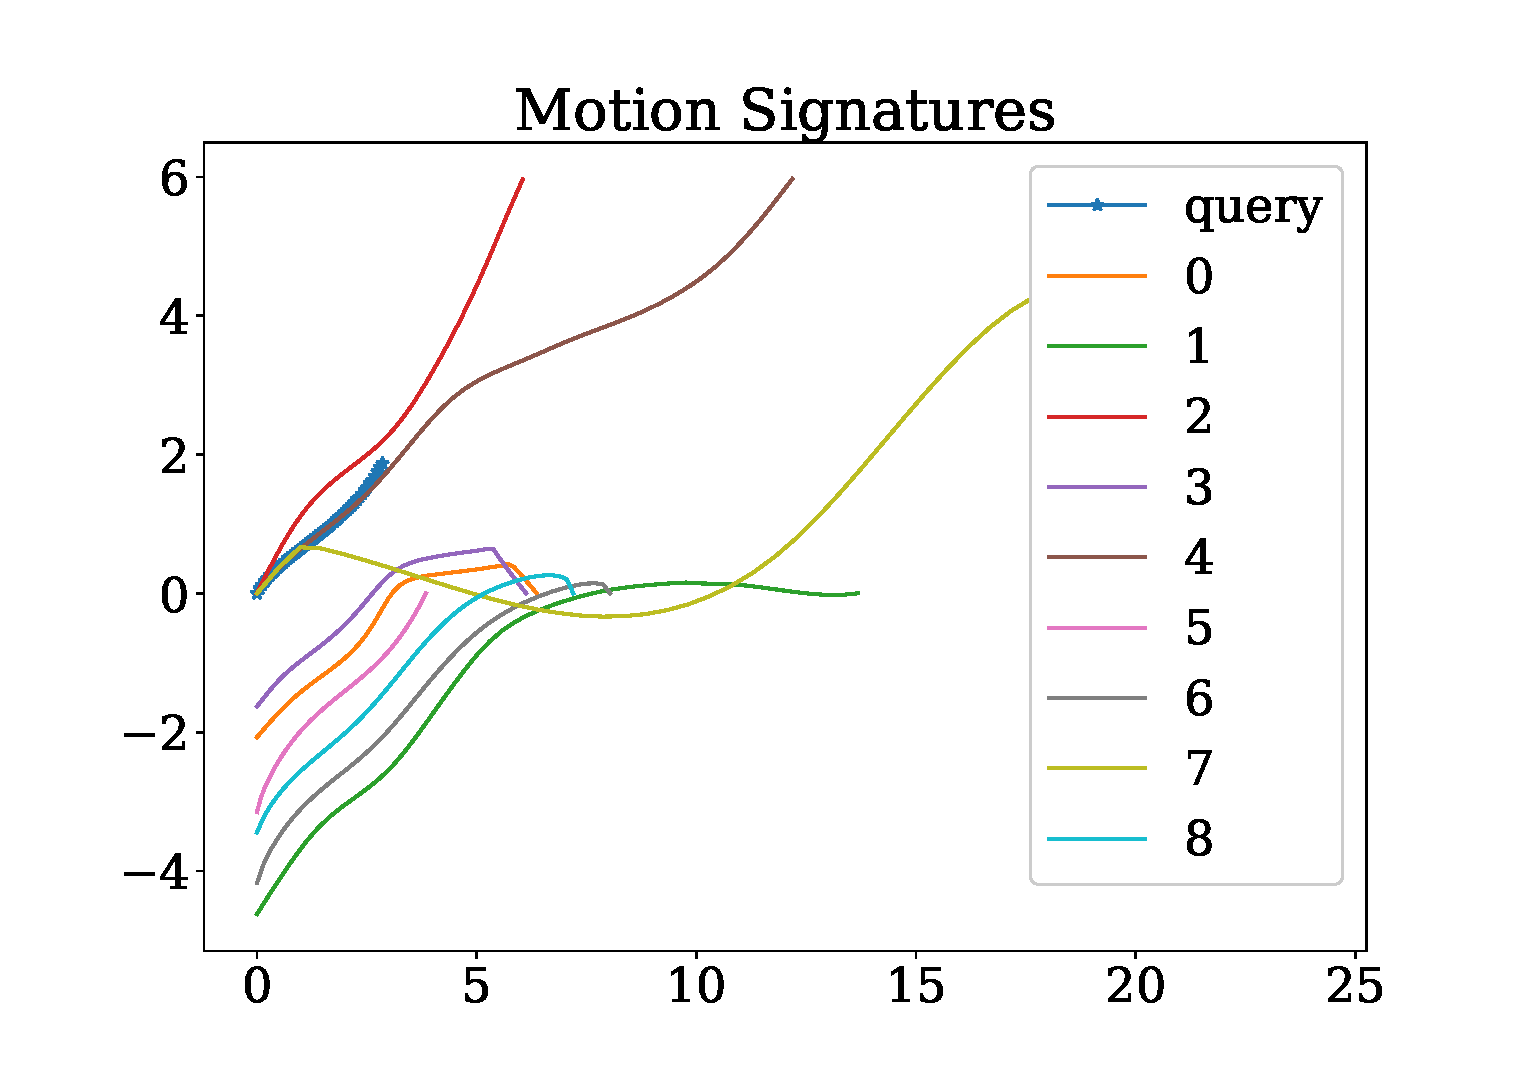
\includegraphics[width=260pt]{figure/fig_ex_motion_signatures.eps}
  \caption{Case Study 2 - Query Result: Motion signatures in the dataset with highest similarity.}
\label{queryResult}
\end{figure}

\begin{figure}
\begin{tabular}{cc}
  1)\putindeepbox[2pt]{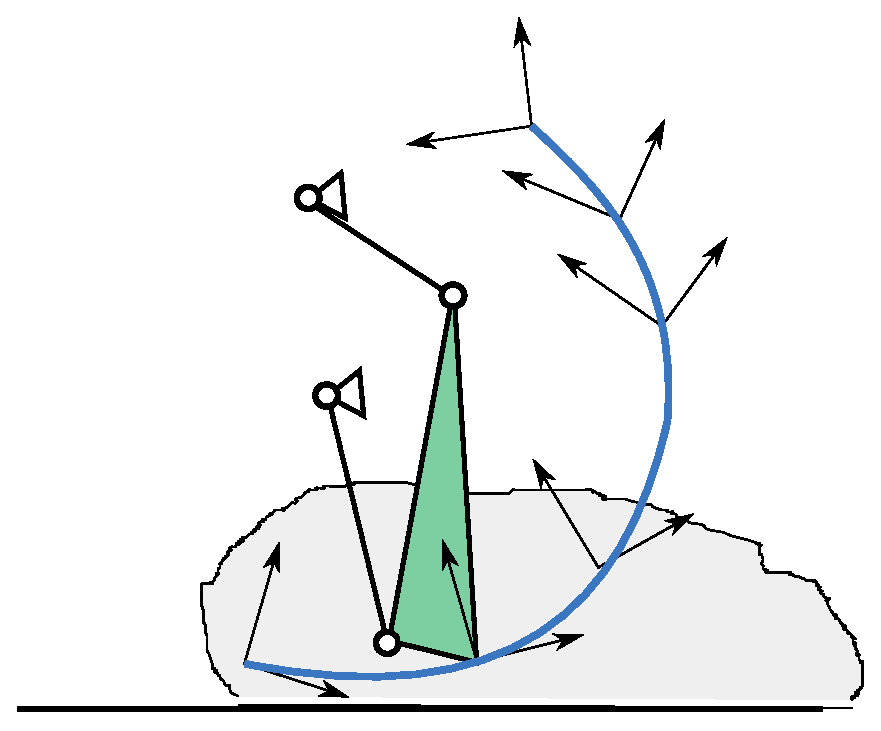
\includegraphics[width=120pt]{figure/sol1.eps}}
    & 2)\putindeepbox[2pt]{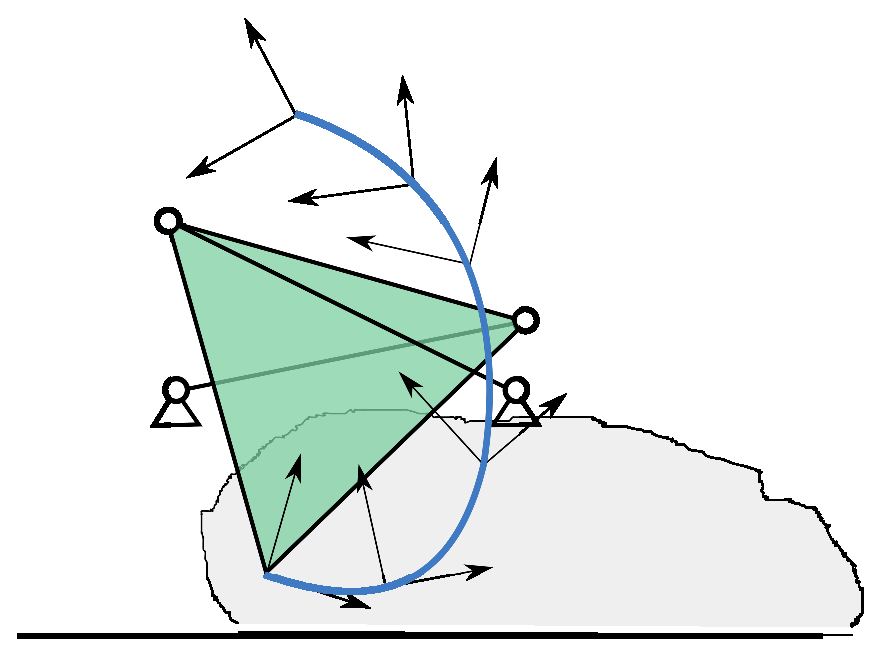
\includegraphics[width=120pt]{figure/sol2.eps}} \\
  3)\putindeepbox[2pt]{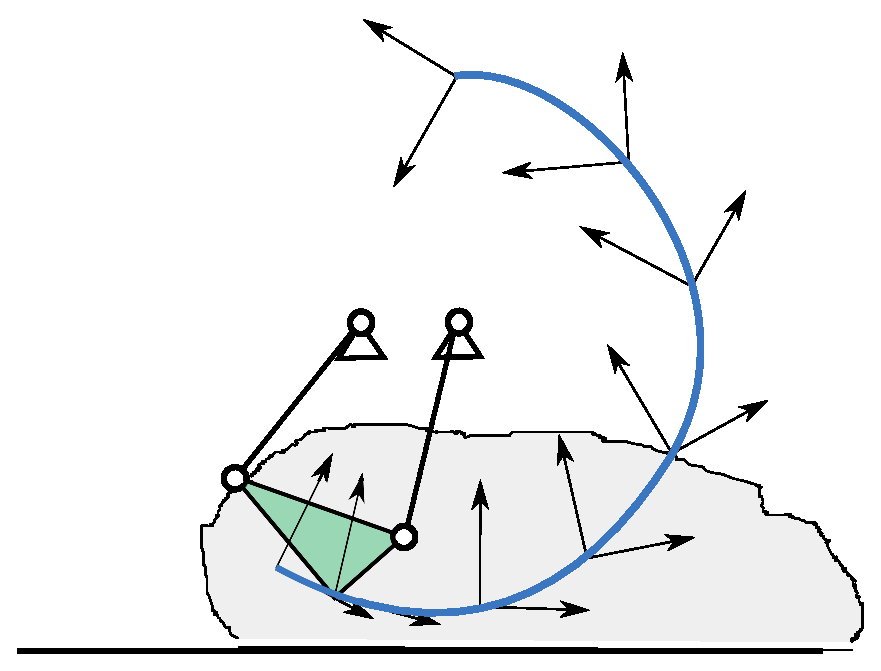
\includegraphics[width=120pt]{figure/sol3.eps}}
    & 4)\putindeepbox[2pt]{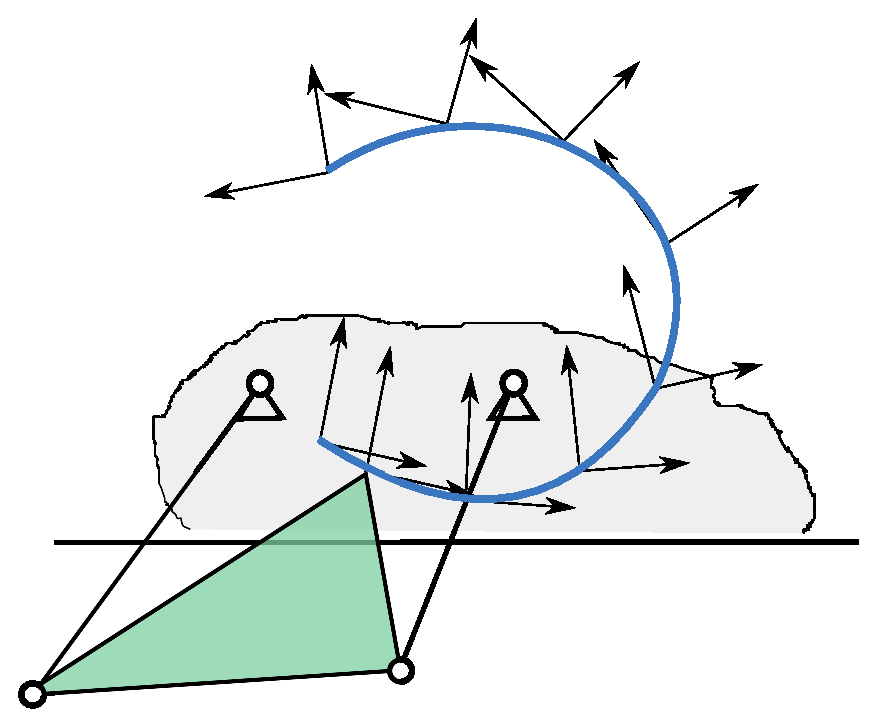
\includegraphics[width=120pt]{figure/sol4.eps}}\\
  5)\putindeepbox[2pt]{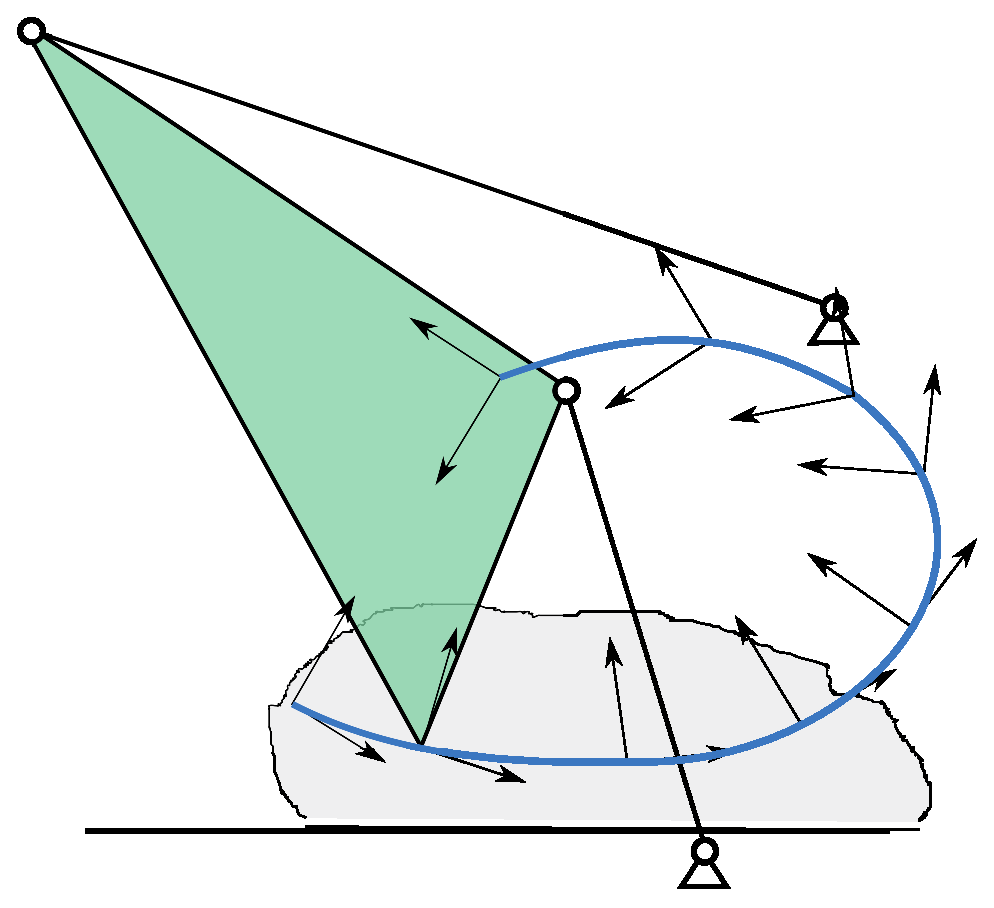
\includegraphics[width=120pt]{figure/sol6.eps}}
    & 6)\putindeepbox[2pt]{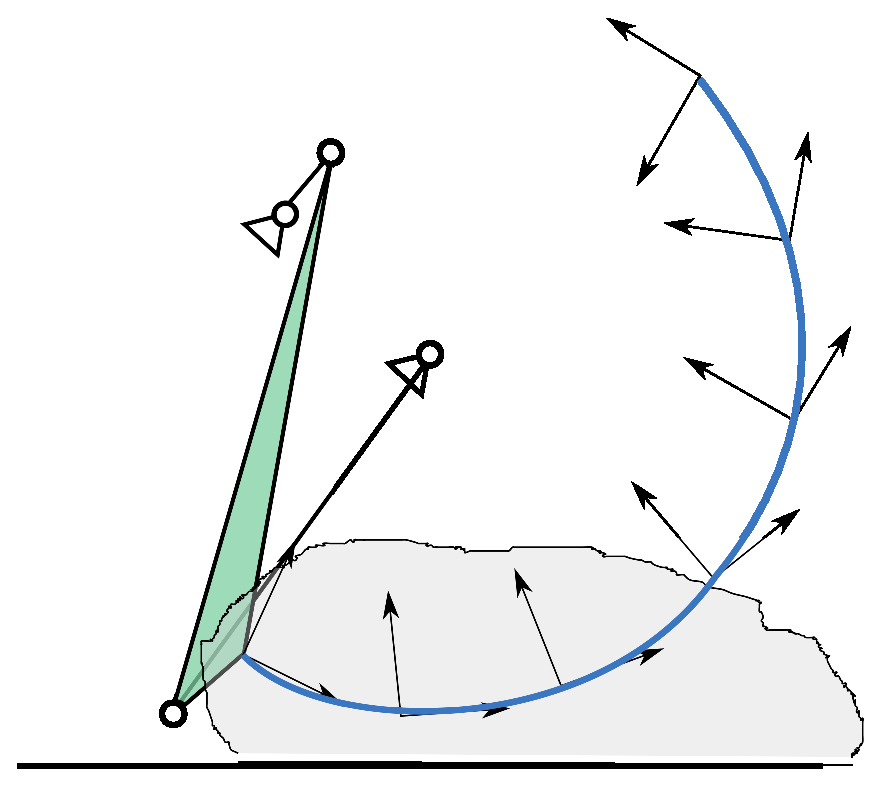
\includegraphics[width=120pt]{figure/sol7.eps}} \\
  7)\putindeepbox[2pt]{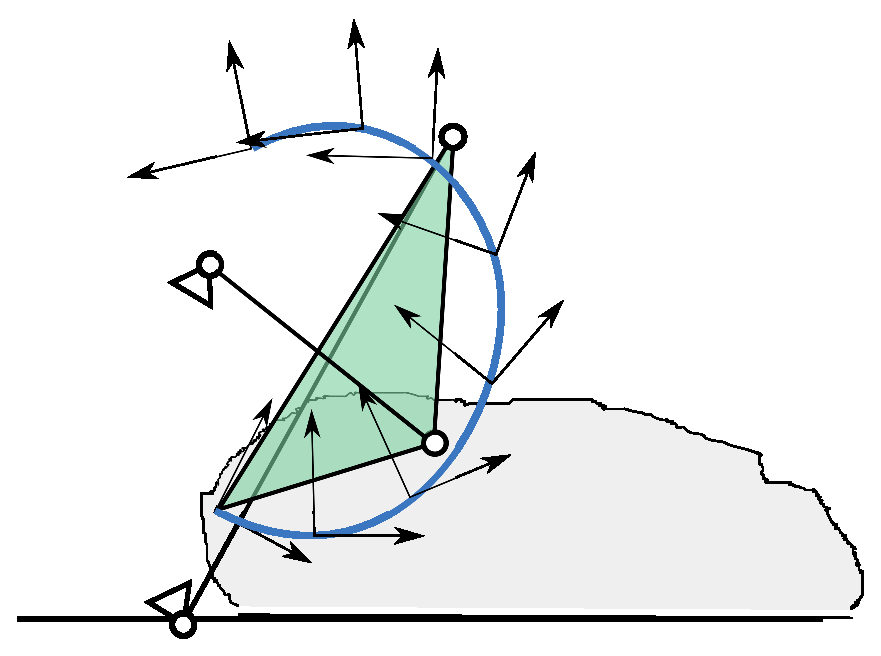
\includegraphics[width=120pt]{figure/sol8.eps}}
    & 8)\putindeepbox[2pt]{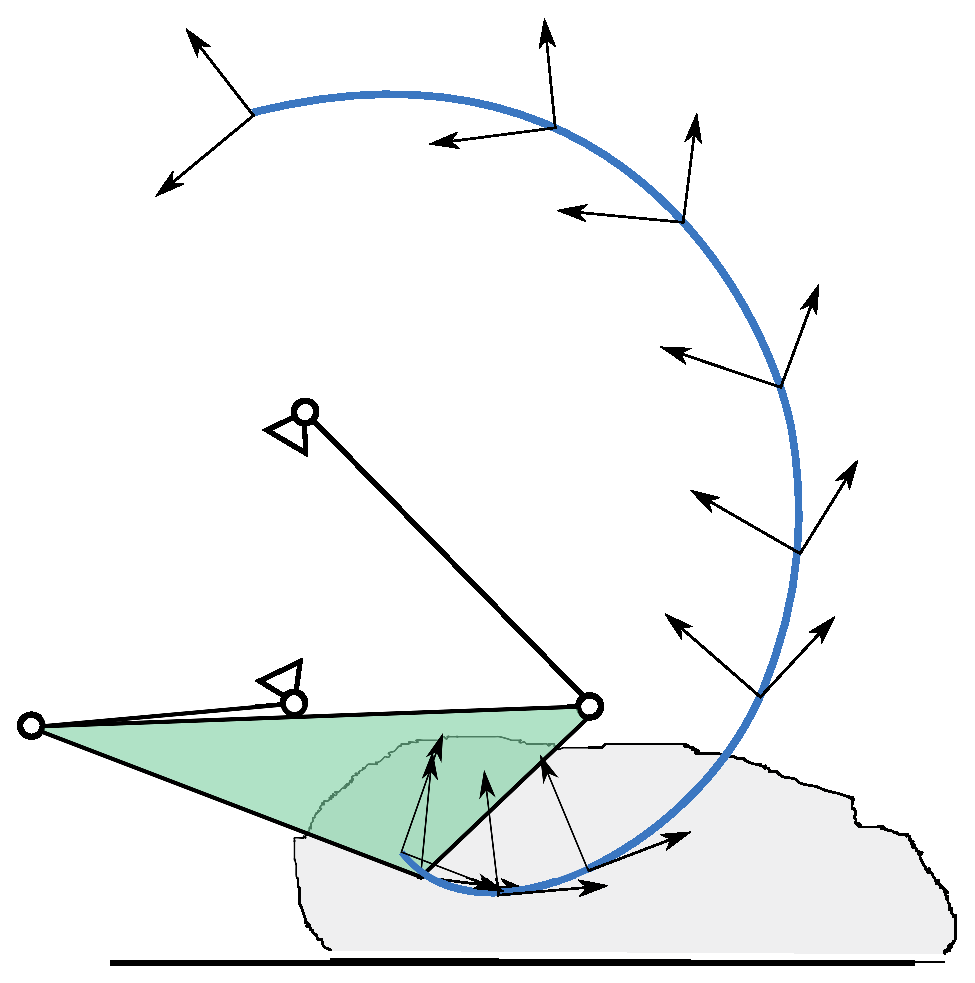
\includegraphics[width=120pt]{figure/sol9.eps}}\\
\end{tabular}
\caption{Case Study 2: First eight linkages in the table~\ref{ex2_knnLinkageData} and their resultant coupler motions.}
\label{ex2_solns}
\end{figure}

The task is to find a pool of linkage systems that can perform snow-shoveling with a motion shown in Fig.~\ref{motionQuery}.
The motion data is tabulated in Table ~\ref{poseData} to which we fit a B-spline with cord length parametrization in order to get the parametric representation of motion.
The task can also be treated as a finite position motion generation and solved for valid solutions.
We try with our real-time computational methods of algebraic fitting\cite{generalfitting-JCISE},\cite{shrinathpurwar2017} but obtained solutions suffer from circuit defect, which is not surprising as those methods do not account for the continuity of input positions.
Also, It is obvious that the coupler should not drop the snow during its entire motion except at the end.
Although the prescribed motion entails this information, precision point approach cannot capture it.

Now we employ the approach presented in this paper.
The first step is to calculate the motion signature of the task motion using steps mentioned in Algorithm ~\ref{alg_signature}.
For that, we follow the steps given in section~\ref{sec_sign} to obtain the motion signature depicted in Fig.~\ref{queryResult}.
Next, we raise the signature query for nearest signatures among cluster centers of the database.
Fig.~\ref{queryResult} shows nine nearest neighbor signatures along with the task signature.
Table~\ref{ex2_knnLinkageData} presents the linkage parameters corresponding to the nearest neighbors along with their distance score from the task.
Coupler motions of these linkages have a part, which matches with the shape of the input motion query.
Actual scaling and orientation of the linkage can be found out easily by comparing analogous points, which are given by the offset index $j$ that corresponds to minimum distance$(E_{min})$ in Eq.~\req{mccEq}.
Figure~\ref{ex2_solns} depict the solutions obtained after scaling and orienting the linkage to match required motion.
All of these linkages satisfactorily perform the input task without any defect.
As ground or fixed pivot locations should lie above the ground, all solutions except the $4^{th}$ solution are suitable for the task.
Although Fig.~\ref{ex2_solns} shows that $5^{th}$ and $7^{th}$ solution may slightly interfere with the ground, it can be rectified by lifting the mechanism slightly up or making small changes in coupler dimensions.
In light of these results, we can say that this approach produces a large variety of solutions, which otherwise would be very hard to find using the precision point approach.


\begin{table}
\caption{Case Study 2: Pose Data}
\centering
\label{poseData}
\begin{tabular}{cccccccc}
\hline
%Pose & x & y & $\theta$ \\
Pose & x & y & $\theta$ & Pose & x & y & $\theta$ \\
\hline
1 & 0.03 & 0.07 & 6.06 & 6 & 1.39 & 0.47 & 0.73 \\
2 & 0.38 & 0.01 & 6.18 & 7 & 1.36 & 0.77 & 1.03 \\
3 & 0.71 &-0.00 & 0.04 & 8 & 1.18 & 1.06 & 1.36 \\
4 & 1.02 & 0.06 & 0.22 & 9 & 0.88 & 1.27 & 1.74 \\
5 & 1.26 & 0.22 & 0.46 & \\
\end{tabular}
\end{table}

\begin{table}
\caption{Case Study 2: Linkage Parameters corresponding to Nine Nearest Neighbor Motions}
\centering
\label{ex2_knnLinkageData}
\begin{tabular}{ccccccc}
\hline
  linkage & $l_1$ & $l_2$ & $l_3$ & $l_4$ & $l_5$ & $E_{min}$ \\
\hline
 1 & 1.28 & 0.88 & 1.77 & -1.32 & 1.79 & 0.0186   \\
 2 & 1.05 & 1.14 & 1.09 & 0.35 & -0.60 & 0.0362   \\
 3 & 2.06 & 2.28 & 1.84 & -1.71 & 0.51 & 0.0378   \\
 4 & 1.52 & 1.22 & 1.46 & 0.05 & 0.12 & 0.0402    \\
 5 & 1.12 & 0.99 & 0.57 & 0.05 & 0.68 & 0.0467    \\
 6 & 1.58 & 0.88 & 1.17 & 0.08 & -0.22 & 0.0481   \\
 7 & 2.17 & 0.38 & 2.87 & -3.51 & 1.39 & 0.0578   \\
 8 & 1.55 & 0.79 & 0.85 & -0.80 & -0.52 & 0.0585  \\
 9 & 0.91 & 1.40 & 1.93 & -0.93 & -0.83 & 0.0605
\end{tabular}
\end{table}




\section*{Conclusion}
The methods based on precision point approach do not capture continuity of the task.
This causes the solutions to have the branch, circuit and order defects.
Also, the formulation fails to detect undesired properties of the coupler motion in the region between precision points.
Thus, we present a perceptive problem formulation, by considering the entire prescribed task.
We solve the proposed formulation by employing machine-learning techniques and generate a large number of defect-free conceptual designs.
The approach is highly data-efficient due to similarity invariant representation and partial matching.
Sensitivity analysis indicates that the complexity of the objective function is well behaved at the singular locations.
The hierarchically clustered database provides an efficient query search.
Finally, the effectiveness of the presented approach is showcased by two case studies.
Every solution presented in the examples section is a result of part-to-whole matching.
The other atlas-based approaches facilitate only whole-to-whole matching, hence they would need a very large amount of data to find these results.

Although the partial matching metric is more accurate, it is expensive in terms of computation cost.
Thus, we use the Euclidean metric in the latent space of compressed data for the hierarchical clustering of the database.
The problem formulation is invariant with respect to translation, orientation, and scaling.
Hence, constraints like geometric restrictions on pivots have to be addressed after finding feasible solutions for the task.
The approach is general enough to be extended to higher order linkage systems for which there are even fewer methods available for synthesizing defect-free solutions.
However, the database size increases exponentially with the number of links in the mechanisms.
As an example, a Watt type six-bar database needs to be roughly 400 times larger than the four-bar database.
A potential solution to this problem could be to use learning based methods, where the pattern is learned instead of storing all of the information.
Overall, the method provides a holistic approach towards the prescribed path and motion synthesis and encourages artificial intelligence techniques to make an impact.


\begin{acknowledgment}
This work has been financially supported by The National Science Foundation under a research grant to Stony Brook University (A. Purwar and Q.J. Ge, grant CMMI-1563413). All findings and results presented in this paper are those of the authors and do not represent those of the funding agencies.
\end{acknowledgment}

\bibliographystyle{purwar}
\bibliography{References}
\newpage
\clearpage
%\listoftables
%\listoffigures

\end{document}
